\documentclass[a4paper, 12pt, UTF8]{ctexart}
\usepackage{amsmath}
\usepackage{amssymb}
\usepackage{booktabs}
\usepackage{graphicx}
\usepackage{listings}
\usepackage{multicol}
\usepackage{longtable}
\usepackage{xcolor}
\usepackage{minted}
\usepackage{enumitem}
\usepackage{geometry}
\geometry{tmargin=.75in, bmargin=.75in, lmargin=.75in, rmargin = .75in}
\graphicspath{{figures/}}
\usepackage{float}
\usepackage{subfig}
\captionsetup[figure]{labelsep=space}  

\lstdefinestyle{cstyle}{
    language=C,
    backgroundcolor=\color{gray!10},
    basicstyle=\ttfamily\small,
    keywordstyle=\color{blue},
    commentstyle=\color{green!50!black},
    stringstyle=\color{red},
    numbers=left,
    numberstyle=\tiny\color{gray},
    stepnumber=1,
    numbersep=5pt,
    showspaces=false,
    showstringspaces=false,
    showtabs=false,
    tabsize=2
}

\setminted{
    fontsize=\footnotesize,
    breaklines
}
\usemintedstyle{xcode}
\usepackage{titlesec}
\usepackage{titletoc}


\setcounter{tocdepth}{3}
\title{CSAPP笔记}
\author{apl}
\date{\today}
\usepackage{hyperref}
\hypersetup{
colorlinks=true,
linkcolor=black
}

\begin{document}
\maketitle

\tableofcontents
\clearpage
\section{环境与工具}
\subsection{Linux操作系统}
\subsubsection{什么是操作系统}
现代计算机由一个或多个处理器、主存、磁盘以及各种输入输出设备组成。操作系统是管理这些组件,并将硬件抽象为统一软件接口的一层软件。
\subsubsection{用户和用户组}
Linux系统是多用户多任务的分时操作系统。根用户账号是\mintinline{bash}{root},拥有最高管理权限,为系统安全通常不直接使用根用户登录。每个用户都属于一个用户组,系统可对用户组中的用户进行集中管理。

\subsubsection{文件和目录权限}
在Linux中,文件和目录具有访问权限。每个文件包含九个权限位,分别定义所有者、所有者所在用户组和其他用户的访问权限。
\begin{minted}{bash}
-rwxr--r-- 1 user user 54130 Jan 8 12:14 README.md
\end{minted}
最前面的 \mintinline{bash}{-} 表示文件,\mintinline{bash}{d} 表示目录,\mintinline{bash}{l} 表示符号链接,后面九位每三位为分隔,\mintinline{bash}{r} 表示读取,\mintinline{bash}{w} 表示写入,\mintinline{bash}{x} 表示执行,\mintinline{bash}{-} 表示无权限。


\subsubsection{文件和目录操作命令}
\begin{enumerate}[label=\arabic*.]
    \item \textbf{\mintinline{bash}{ls}命令}:用于列出指定目录下的子目录及文件名称,格式为\mintinline{bash}{ls [选项] 路径},如\mintinline{bash}{ls -a}可连同隐藏文件一起列出,\mintinline{bash}{ls -l}可列出文件和目录的属性与权限等详细数据。
    \item \textbf{\mintinline{bash}{cd}命令}:改变当前工作目录,格式为\mintinline{bash}{cd 路径}。
    \item \textbf{\mintinline{bash}{pwd}命令}:显示当前工作目录。
    \item \textbf{\mintinline{bash}{mkdir}命令}:创建新的目录,格式为\mintinline{bash}{mkdir [选项] 路径},\mintinline{bash}{-p}可同时创建多级目录,如\mintinline{bash}{mkdir -p /home/user/documents/work/project}。
    \item \textbf{\mintinline{bash}{rmdir}命令}:删除空的目录,格式为\mintinline{bash}{rmdir [选项] 路径}。
    \item \textbf{\mintinline{bash}{cp}命令}:复制文件或目录,格式为\mintinline{bash}{cp [选项] 源路径1 源路径2 …… 源路径n 目标路径},\mintinline{bash}{-r}选项用于递归复制目录下的所有子文件和子文件夹,\mintinline{bash}{-f}选项可强行覆盖目标文件。
    \item \textbf{\mintinline{bash}{rm}命令}:删除文件或目录,格式为\mintinline{bash}{rm [选项] 路径1 路径2 …… 路径n},删除文件夹需使用\mintinline{bash}{-r}选项,\mintinline{bash}{-f}选项可强行删除目标文件。
    \item \textbf{\mintinline{bash}{mv}命令}:移动文件与目录,格式为\mintinline{bash}{mv 源路径1 源路径2 …… 源路径n 目标路径},也可用于文件重命名,如\mintinline{bash}{mv file1 file5}把file1重命名为file5。
    \item \textbf{\mintinline{bash}{chmod}命令}:改变文件权限,格式为\mintinline{bash}{chmod 模式 路径},模式如\mintinline{bash}{[ugoa...][[+-=][rwx]...]},\mintinline{bash}{u}表示文件拥有者,\mintinline{bash}{g}表示同用户组,\mintinline{bash}{o}表示其他用户,\mintinline{bash}{a}表示三者皆是,\mintinline{bash}{+}增加权限,\mintinline{bash}{-}取消权限,\mintinline{bash}{=}唯一设定权限。
    \item \textbf{\mintinline{bash}{ln}命令}:创建文件链接,格式为\mintinline{bash}{ln [选项] 源路径 目标路径}。Linux系统允许创建文件链接,分为硬链接(类似文件别名)和软链接(类似快捷方式)。\mintinline{bash}{-s}选项用于创建软链接,\mintinline{bash}{-f}选项可强制执行。
    \item \textbf{\mintinline{bash}{tar}命令}:文件打包和拆包,如\mintinline{bash}{tar czf file.tar.gz file/}可将\mintinline{bash}{file}文件夹下的所有内容压缩为\mintinline{bash}{file.tar.gz},使用\mintinline{bash}{gzip}压缩算法。如\mintinline{bash}{tar xzf file.tar.gz}可将\mintinline{bash}{file.tar.gz}解压缩到当前文件夹(拆包时参数\mintinline{bash}{z}可省略)。
          \begin{table}[H]
              \captionsetup{skip=4pt}
              \centering
              \setlength{\arrayrulewidth}{1pt}
              \begin{tabular}{ccc}
                  \hline
                  \makebox[0.2\textwidth][c]{压缩算法} & \makebox[0.1\textwidth][c]{参数} & \makebox[0.2\textwidth][c]{后缀} \\
                  \noalign{\global\setlength{\arrayrulewidth}{0.5pt}}
                  \hline
                  gzip                             & z                              & .tar.gz                        \\
                  bzip2                            & j                              & .tar.bz2                       \\
                  Lempress-Ziv                     & Z                              & .tar.Z                         \\

                  \noalign{\global\setlength{\arrayrulewidth}{1pt}}
                  \hline
              \end{tabular}
              \caption{几种常见压缩算法参数}
          \end{table}
    \item \textbf{\mintinline{bash}{zip/unzip}命令}:文件打包和解包,如\mintinline{bash}{zip -q -r html.zip /home/html}和\mintinline{bash}{unzip html.zip}。
    \item \textbf{\mintinline{bash}{cat}命令}:将文件以文本方式输出至控制台。
    \item \textbf{\mintinline{bash}{hexdump}命令}:将文件以编码形式输出至控制台。
    \item \textbf{\mintinline{bash}{head}命令}:显示文件前几行的数据。
    \item \textbf{\mintinline{bash}{tail}命令}:输出文件尾部的数据。
    \item \textbf{\mintinline{bash}{objdump}命令}:查看\mintinline{bash}{elf}格式文件。
    \item \textbf{\mintinline{bash}{more}命令}:分页显示文件
    \item \textbf{\mintinline{bash}{find}命令}:根据条件搜索文件,如\mintinline{bash}{find ./test1 –name a.txt}可在当前目录下的\mintinline{bash}{test1}子目录中搜索\mintinline{bash}{a.txt}文件。
    \item \textbf{\mintinline{bash}{grep}命令}:根据条件搜索文件内容(常用于搜索文本文件),如\mintinline{bash}{grep hello file.txt}可在\mintinline{bash}{file.txt}中查找字符串\mintinline{bash}{hello}并打印匹配的行。
\end{enumerate}

\subsection{文本编辑器vi/vim}

\subsubsection{VIM的工作模式}
\begin{enumerate}
    \item 普通模式:用于导航、删除、复制等,是默认模式
    \item 查找模式:用于搜索文本
    \item 插入模式:用于输入文本
    \item 命令模式:用于执行保存、退出等高级命令
    \item 可视模式:用于选择文本块
\end{enumerate}

\begin{figure}[H]
    \centering
    \captionsetup{skip=4pt}
    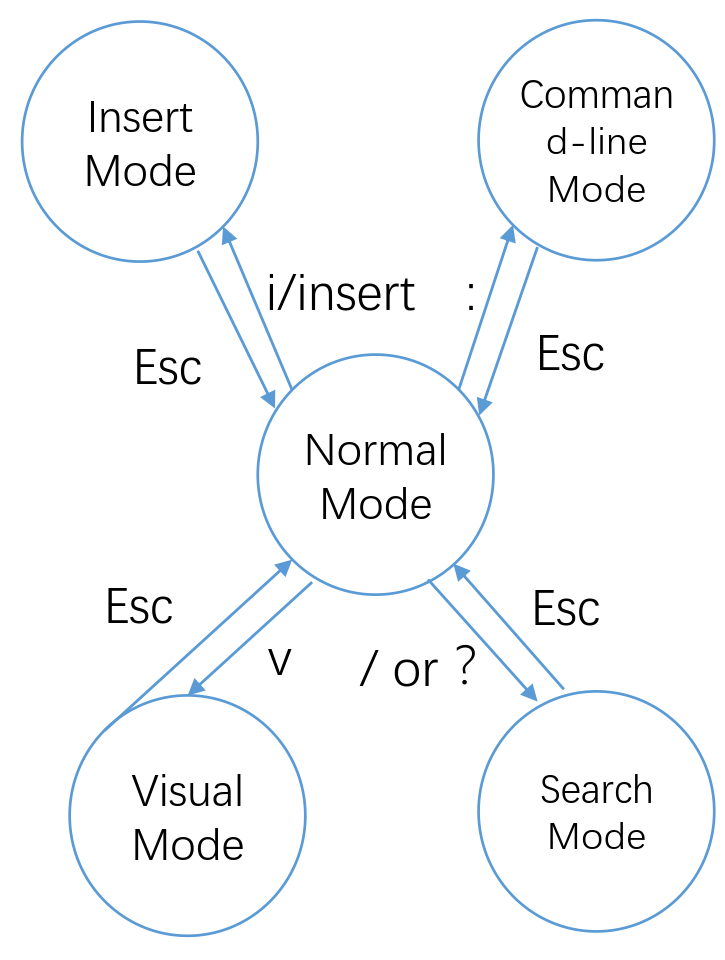
\includegraphics[width=5cm]{5.png}
    \caption{vim的工作模式}
\end{figure}

\subsubsection{各模式下的操作}
\begin{enumerate}[label=\arabic*.]
    \item \textbf{普通模式}:可使用上下左右键、\mintinline{bash}{Home}、\mintinline{bash}{End}、\mintinline{bash}{PageUp}、\mintinline{bash}{PageDown}、\mintinline{bash}{gg}、\mintinline{bash}{Shift + g}等键移动光标,\mintinline{bash}{yy}复制当前行,\mintinline{bash}{dd}剪切当前行,\mintinline{bash}{p}粘贴,\mintinline{bash}{u}撤销,\mintinline{bash}{Ctrl + r}恢复撤销操作。
    \item \textbf{插入模式}:按\mintinline{bash}{i}键或\mintinline{bash}{Insert}键进入,支持方向键等移动光标,按\mintinline{bash}{Insert}键可切换插入和替换模式。
    \item \textbf{查找模式}:按\mintinline{bash}{/}或\mintinline{bash}{?}键进入,输入查找字符串并回车查找,按\mintinline{bash}{n}键查找下一项,\mintinline{bash}{Shift + n}查找上一项。
    \item \textbf{命令模式}:按\mintinline{bash}{:}键进入,输入\mintinline{bash}{w}保存,\mintinline{bash}{q}退出,\mintinline{bash}{wq}保存并退出等命令。
    \item \textbf{可视模式}:按\mintinline{bash}{v}键进入,移动光标选择文本块,\mintinline{bash}{y}键复制,\mintinline{bash}{d}键剪切,普通模式下\mintinline{bash}{p}键粘贴。
\end{enumerate}

\subsection{GNU工具链}
\subsubsection{GNU工具链简介}
GNU工具链是一组开源编程工具,由GNU计划提供,包含用于编译、调试和构建软件的实用程序,如GCC(支持多种编程语言的编译器集合)、GNU Binutils(包括汇编器、连接器等)、GDB(调试程序的工具)、Make(用于构建和管理项目的工具,通过Makefile文件描述构建规则)。

\subsubsection{构建程序}
\begin{enumerate}[label=\arabic*.]
    \item \textbf{单个源文件}:可使用\mintinline{bash}{gcc main.c}编译并链接\mintinline{c}{main.c},默认生成\mintinline{bash}{a.out};也可使用\mintinline{bash}{gcc -o main main.c}指定生成文件名为\mintinline{bash}{main}。
    \item \textbf{多个源文件}:如编译\mintinline{c}{a.c}和\mintinline{c}{b.c},可使用\mintinline{bash}{gcc a.c b.c -o p}直接编译链接生成\mintinline{bash}{p}文件;也可先\mintinline{bash}{gcc –c a.c b.c}生成目标文件,再\mintinline{bash}{gcc –o p a.o b.o}链接生成\mintinline{bash}{p}文件。
\end{enumerate}

\subsubsection{增量编译}
只编译修改的文件再链接,可提高编译效率。如只编译\mintinline{c}{b.c},使用\mintinline{bash}{gcc –c b.c},再\mintinline{bash}{gcc –o p a.o b.o}链接。

\subsubsection{引用自定义头文件与链接第三方库}
引用自定义头文件时,使用\mintinline{bash}{-I}指定头文件搜索目录,如\mintinline{bash}{gcc –c a.c –Iinc}。链接第三方库时,使用\mintinline{bash}{-l}指定库名称,如\mintinline{bash}{gcc –o p a.o -lm}链接数学库;若库不在默认搜索路径,使用\mintinline{bash}{-L}指定路径。

\subsubsection{自动化编译}
\begin{enumerate}[label=\arabic*.]
    \item \textbf{编写shell脚本}:编写脚本可简化编译过程,但存在局限性,如处理复杂项目时脚本复杂、无法增量编译等。
    \item \textbf{使用Makefile}:在工程根目录创建Makefile文件,编写规则后使用\mintinline{bash}{make}命令编译。Makefile中可定义变量,如\mintinline{bash}{CC}(编译器)、\mintinline{bash}{CFLAGS}(编译选项)等,规则包含目标、依赖和命令,\mintinline{bash}{make}会根据依赖关系和时间戳确定编译操作。
\end{enumerate}

\subsubsection{在编译程序时增加调试信息}
编译时添加\mintinline{bash}{-g}选项,如\mintinline{bash}{CFLAGS = -Iinc -g},可使编译器在生成目标文件时包含调试信息,便于使用GDB调试程序,如设置断点、查看变量值等。


\subsection{代码版本管理}

\subsubsection{Git的基本概念}
包括仓库(项目的版本控制库,可在本地或远程服务器)、提交(对代码库的保存,包含代码修改等)、暂存区(文件提交前的临时区域)、还原(用仓库记录还原工作目录文件更改)、推送(将本地仓库更改上传到远程仓库)、拉取(从远程仓库获取最新更改并应用到本地仓库)。

\subsubsection{创建本地仓库与提交文件}
使用\mintinline{bash}{mkdir}创建本地工作目录,\mintinline{bash}{cd}进入目录,\mintinline{bash}{git init}创建空的本地仓库。创建文件后使用\mintinline{bash}{git add}将文件转换为staged状态,再用\mintinline{bash}{git commit}提交至版本库,提交时可编辑提交说明。

\subsubsection{查看提交日志与代码还原}
使用\mintinline{bash}{git log}命令可查看提交日志,包含提交记录标识、作者、日期和提交说明等信息。使用\mintinline{bash}{git restore}命令可进行代码还原,如\mintinline{bash}{git restore main.c}用最近一次提交覆盖工作区文件,也可指定提交记录标识还原。

\subsubsection{远程仓库操作}
以GITEE为例,可创建空的远程仓库,使用\mintinline{bash}{git remote add origin 远程仓库地址}关联远程仓库,首次推送使用\mintinline{bash}{git push -u origin master},后续只需\mintinline{bash}{git push}。也可使用\mintinline{bash}{git clone}命令克隆远程仓库至本地。

\subsubsection{多人协作开发}
多人协作开发时,开发者克隆远程仓库至本地,各自进行代码修改后提交。推送前需先拉取远程仓库最新代码,若有冲突需解决冲突后再推送。冲突多数可由git自动解决,无法自动解决时需人工干预编辑冲突区域代码。

\section{信息的存储}
\subsection{使用比特表示信息}
\subsubsection{万物皆比特}
由于信号易存储在双稳态单元中,并且可以在存在噪声和不准确的信道中可靠地传输。信息都可以使用二进制的编码进行表示,计算机通过二进制来发送指令,以及表示和处理各种数字、字符串等。

\subsubsection{字节数据编码}
1 Byte = 8 bits。二进制表示范围是 \(00000000_{2}\) 到 \(11111111_{2}\);十进制表示范围是 \(0_{10}\) 到 \(255_{10}\);十六进制表示范围是 \(00_{16}\) 到 \(FF_{16}\),十六进制以 16 为基数,计数符号为 0 - 9 和 A - F 。在 C 语言中,FA1D37B$_{16}$ 可表示为 0xFA1D37B 或 0xfa1d37b。
\begin{table}[H]
    \captionsetup{skip=4pt}
    \centering
    \setlength{\arrayrulewidth}{1pt}
    \begin{tabular}{ccc}
        \hline
        \makebox[0.2\textwidth][c]{十进制} & \makebox[0.2\textwidth][c]{十六进制} & \makebox[0.2\textwidth][c]{二进制} \\
        \noalign{\global\setlength{\arrayrulewidth}{0.5pt}}
        \hline
        0                               & 00                               & 00000000                        \\
        1                               & 01                               & 00000001                        \\
        2                               & 02                               & 00000010                        \\
        3                               & 03                               & 00000011                        \\
        4                               & 04                               & 00000100                        \\
        5                               & 05                               & 00000101                        \\
        6                               & 06                               & 00000110                        \\
        7                               & 07                               & 00000111                        \\
        8                               & 08                               & 00001000                        \\
        9                               & 09                               & 00001001                        \\
        10                              & 0A                               & 00001010                        \\
        11                              & 0B                               & 00001011                        \\
        12                              & 0C                               & 00001100                        \\
        13                              & 0D                               & 00001101                        \\
        14                              & 0E                               & 00001110                        \\
        15                              & 0F                               & 00001111                        \\
        \noalign{\global\setlength{\arrayrulewidth}{1pt}}
        \hline
    \end{tabular}
    \caption{字节数据编码对应表}
\end{table}
\subsection{位运算}
\subsubsection{布尔代数}
\begin{itemize}
    \item And(与):\(A \& B = 1\) 当且仅当 \(A = 1\) 且 \(B = 1\)。
    \item Or(或):\(A | B = 1\) 当 \(A = 1\) 或者 \(B = 1\)。
    \item Not(非):\(\sim A = 1\) 当 \(A = 0\)。
    \item Exclusive - Or(Xor,异或):\(A\^{}B = 1\) 当 \(A = 1\) 或者 \(B = 1\),但不同时为 1,即相同为 0,不同为 1。
\end{itemize}

\subsubsection{C 语言中的位运算}
C 语言定义了四个位运算符号:
\begin{table}[H]
    \captionsetup{skip=4pt}
    \centering
    \setlength{\arrayrulewidth}{1pt}
    \begin{tabular}{cccc}
        \hline
        \makebox[0.15\textwidth][c]{C 表达式} & \makebox[0.2\textwidth][c]{二进制表达式} & \makebox[0.2\textwidth][c]{二进制结果} & \makebox[0.15\textwidth][c]{十六进制结果} \\
        \noalign{\global\setlength{\arrayrulewidth}{0.5pt}}
        \hline
        $\sim$ 0x41                        & $\sim$[0100 0001]                  & \([10111110]\)                    & 0xBE                                \\
        $\sim $ 0x00                       & \(\sim[0000 0000]\)                & \([11111111]\)                    & 0xFF                                \\
        0x69\&0x55                         & \([0110 1001]\&[0101 0101]\)       & \([0100 0001]\)                   & 0x41                                \\
        0x69 | 0x55                        & \([0110 1001] | [0101 0101]\)      & \([01111101]\)                    & 0x7D                                \\
        \noalign{\global\setlength{\arrayrulewidth}{1pt}}
        \hline
    \end{tabular}
    \caption{C 语言位运算示例}
\end{table}
\subsubsection{异或运算的应用:数据交换}
在 C 语言中,可以利用异或运算实现不使用额外变量交换两个数:
\begin{minted}{c}
void funny(int *x, int *y)
{
    *x = *x ^ *y; /* #1 */
    *y = *x ^ *y; /* #2 */
    *x = *x ^ *y; /* #3 */
}
\end{minted}
交换过程如下:
\begin{table}[H]
    \captionsetup{skip=4pt}
    \centering
    \setlength{\arrayrulewidth}{1pt}
    \begin{tabular}{ccc}
        \hline
        \makebox[0.1\textwidth][c]{步骤} & \makebox[0.2\textwidth][c]{*x}                     & \makebox[0.2\textwidth][c]{*y}     \\
        \noalign{\global\setlength{\arrayrulewidth}{0.5pt}}
        \hline
        开始                             & A                                                  & B                                  \\
        1                              & A\^{}B                                             & B                                  \\
        2                              & A\^{}B                                             & (A\^{}B)\^{}B = A\^{}(B\^{}B) =  A \\
        3                              & (A\^{}B)\^{}A = (B\^{}A)\^{}A = B\^{}(A\^{}A)  = B & A                                  \\
        结束                             & B                                                  & A                                  \\
        \noalign{\global\setlength{\arrayrulewidth}{1pt}}
        \hline
    \end{tabular}
    \caption{异或运算交换数据过程}
\end{table}
\subsubsection{C 语言中的逻辑运算}
C 语言定义了三种逻辑运算:\(||\)(逻辑或)、\&\&(逻辑与)、\(!\)(逻辑非),具有短路效应。例如:
\begin{itemize}
    \item x \&\& 5/x 可以用于避免除 0 运算。
    \item p \&\& *p++ 可以避免空指针运算。
    \item 5 || x = y 赋值语句将不会被执行。
\end{itemize}
\subsubsection{C 语言中的移位运算}
C 语言中有逻辑移位和算术移位。右移运算有逻辑移位(左侧补 0)和算术移位(左侧补原最高位值)两种操作。对于无符号数,右移是逻辑的;对于有符号数,几乎所有的编译器针对有符号数的右移都采用的是算术右移
\begin{figure}[H]
    \centering
    \captionsetup{skip=4pt}
    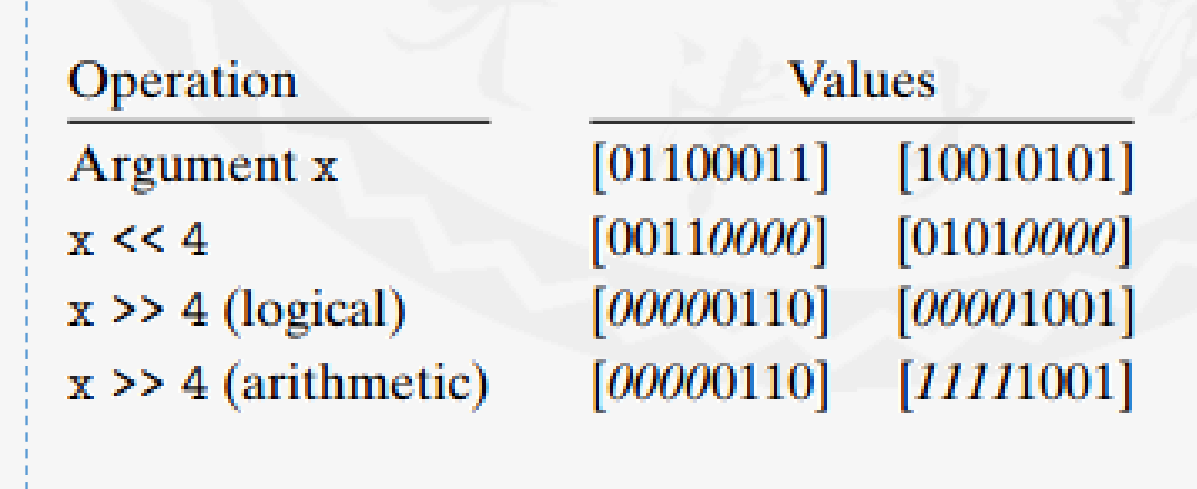
\includegraphics[width=6cm]{3.png}
    \caption{移位运算}
\end{figure}
\subsubsection{未定义行为}
C 语言规范中没有被明确定义的行为称为未定义行为(UB),编程时应避免使用未定义行为,但有符号数算术右移除外。例如,移位 \(k\),当 \(k\) 大于等于变量位长时,值直接变为0,在 GCC 中的实现如下:
\begin{minted}{c}
int aval = 0x0EDCBA98 >> 36; 
movl $0, -8(%ebp)   // 值直接变为0
unsigned uval = 0xFEDCBA98u << 40;
movl $0, -4(%ebp)   // 值直接变为0
\end{minted}
\subsubsection{运算优先级}
移位运算符的优先级低于加减乘除,例如 \(- 1<<2+3<<4\),正确的运算顺序为 \((1<<(2 + 3))<<4\) 。
\subsection{信息的存储和表示}
\subsubsection{字长}
字长是指针数据的大小(虚拟地址宽度)。 32 位 ( 4 字节) 计算机字长限制了地址空间为 4GiB(\(2^{32}\) 字节);64 位字长( 8 字节)寻址能力达到了 18EiB
\subsubsection{C 语言中的各数据类型位宽}
计算机和编译器支持多种数据类型,或是小于字长,或大于字长,但长度都是整数个字节。
\begin{table}[H]
    \captionsetup{skip=4pt}
    \centering
    \setlength{\arrayrulewidth}{1pt}
    \begin{tabular}{cccc}
        \hline
        \makebox[0.15\textwidth][c]{C 语言数据类型} & \makebox[0.15\textwidth][c]{典型 32 位系统} & \makebox[0.15\textwidth][c]{典型 64 位系统} & \makebox[0.15\textwidth][c]{x86 - 64} \\
        \noalign{\global\setlength{\arrayrulewidth}{0.5pt}}
        \hline
        char                                  & 1                                      & 1                                      & 1                                     \\
        short                                 & 2                                      & 2                                      & 2                                     \\
        int                                   & 4                                      & 4                                      & 4                                     \\
        long                                  & 4                                      & 8                                      & 8                                     \\
        float                                 & 4                                      & 4                                      & 4                                     \\
        double                                & 8                                      & 8                                      & 8                                     \\
        pointer                               & 4                                      & 8                                      & 8                                     \\
        \noalign{\global\setlength{\arrayrulewidth}{1pt}}
        \hline
    \end{tabular}
    \caption{C 语言数据类型位宽}
\end{table}
\subsubsection{字节序}
有小端序(Little endian)和大端序(Big endian)两种。小端序如 Intel,低地址存放低位数据,高地址存放高位数据;大端序如 IBM、Sun Microsystem(Oracle),低地址存放高位数据,高地址存放低位数据。例如,对于 0x1234567 :
\begin{table}[H]
    \captionsetup{skip=4pt}
    \centering
    \setlength{\arrayrulewidth}{1pt}
    \begin{tabular}{ccccc}
        \hline
        \multicolumn{5}{|c|}{地址}                                                                                                                                       \\
        \cline{1-5}
        \makebox[0.1\textwidth][c]{} & \makebox[0.1\textwidth][c]{低地址} & \makebox[0.1\textwidth][c]{} & \makebox[0.1\textwidth][c]{} & \makebox[0.1\textwidth][c]{高地址} \\
        \noalign{\global\setlength{\arrayrulewidth}{0.5pt}}
        \hline
        大端序                          & \(0x100: 0x12\)                 & \(0x101: 0x34\)              & \(0x102: 0x56\)              & \(0x103: 0x07\)                 \\
        小端序                          & \(0x100: 0x07\)                 & \(0x101: 0x56\)              & \(0x102: 0x34\)              & \(0x103: 0x12\)                 \\
        \noalign{\global\setlength{\arrayrulewidth}{1pt}}
        \hline
    \end{tabular}
    \caption{字节序示例}
\end{table}
\subsubsection{探索数据在存储器中的存储方式}
通过以下代码可以打印各变量的字节表示形式:
\begin{minted}{c}
#include <stdio.h>
typedef unsigned char *byte_pointer;
void show_bytes(byte_pointer start,int len)
{
    int i;
    for(i = 0; i < len; i++)
        printf("%.2x ",start[i]);
    printf("\n");
}
void show_int(int x)
{
    show_bytes((byte_pointer)&x, sizeof(int));
}
void show_float(float x)
{
    show_bytes((byte_pointer)&x, sizeof(float));
}
void show_pointer(void *x)
{
    show_bytes((byte_pointer)x, sizeof(void*));
}
\end{minted}
在 Linux32/64(小端)、Win32(小端)和 Sun(32 位,大端)系统下的测试结果如下:
\begin{table}[H]
    \captionsetup{skip=4pt}
    \centering
    \setlength{\arrayrulewidth}{1pt}
    \begin{tabular}{cccc}
        \hline
        \makebox[0.1\textwidth][c]{机器} & \makebox[0.1\textwidth][c]{值}           & \makebox[0.1\textwidth][c]{类型} & \makebox[0.2\textwidth][c]{字节(十六进制)} \\
        \noalign{\global\setlength{\arrayrulewidth}{0.5pt}}
        \hline
        Linux 32                       & 12345                                   & int                            & 39 30 00 00                          \\
        Windows                        & 12345                                   & int                            & 39 30 00 00                          \\
        Sun                            & 12345                                   & int                            & 00 00 30 39                          \\
        Linux 64                       & 12345                                   & int                            & 39 30 00 00                          \\
        Linux 32                       & 12345.0                                 & float                          & 00 e4 40 46                          \\
        Windows                        & 12345.0                                 & float                          & 00 e4 40 46                          \\
        Sun                            & 12345.0                                 & float                          & 46 40 e4 00                          \\
        Linux 64                       & 12345.0                                 & float                          & 00 e4 40 46                          \\
        Linux 32                       & \(      \& ival\)                       & int *                          & e4 f9 ff bf                          \\
        Windows                        & \(                            \& ival\) & int *                          & b4 cc 22 00                          \\
        Sun                            & \(                            \& ival\) & int *                          & ef ff fa 0c                          \\
        Linux 64                       & \(                            \& ival\) & int *                          & b8 11 e5 ff ff 7f 00 00              \\
        \noalign{\global\setlength{\arrayrulewidth}{1pt}}
        \hline
    \end{tabular}
    \caption{不同系统下数据存储测试结果}
\end{table}
\subsubsection{指针的存储方法}
不同的编译器和计算机可能会分配不同的地址,甚至每一次运行时得到的结果都不相同。例如,在 x86 - 64、Sun、IA32 环境下:
\begin{minted}{c}
int B = -15213; 
int *P = &B;
\end{minted}
\subsubsection{字符串的表示}
C 语言的字符串使用 char 数组表示,每个字符都被编码成 ASCII 码,是一个 7 比特的字符编码集(扩展集为 8 比特)。字符“0”的编码是 \(0x30\),数字字符 \(i\) 的编码是 \(0x30 + i\) 。字符串的结尾应为空字符,即 ASCII 编码为 0 。字符串的表示与字节序无关,大小端兼容。
\subsubsection{程序的表示}
不同类型的机器使用不同的且不兼容的指令和指令编码。在相同处理器不同的操作系统中,由于编码规范存在差异,同样代码所生成的程序也不是二进制兼容的,程序很少能够在不同类型机器和不同操作系统中实现二进制水平上移植。
\subsubsection{小知识:PE 和 ELF 格式}
Windows 操作系统下常用的可执行文件格式是 PE(Portable Executable);Unix 家族(含 Linux)操作系统下可执行文件格式为 ELF(Executable and Linkable Format)。

\section{整数}
\subsection{编码}
\subsubsection{整数的表示}
不同C语言数据类型在32位和64位机器上有不同的取值范围:
\begin{table}[H]
    \captionsetup{skip=4pt}
    \centering
    \setlength{\arrayrulewidth}{1pt}
    \begin{tabular}{ccc}
        \hline
        \makebox[0.2\textwidth][c]{C语言数据类型} & \makebox[0.2\textwidth][c]{32位机器} & \makebox[0.2\textwidth][c]{64位机器}             \\
        \noalign{\global\setlength{\arrayrulewidth}{0.5pt}}
        \hline
        char                                & $-128\sim 127$                    & $-128\sim127$                                 \\
        unsigned char                       & $0\sim255$                        & $0\sim255$                                    \\
        short                               & $-32768\sim32767$                 & $-32768\sim32767$                             \\
        unsigned short                      & $0\sim65535$                      & $0\sim65535$                                  \\
        int                                 & $-2147483648\sim2147483647$       & $-2147483648\sim2147483647$                   \\
        unsigned int                        & $0\sim4294967295 $                & $0\sim4294967295$                             \\
        long                                & $-2147483648\sim2147483647$       & $-9223372036854775808\sim9223372036854775807$ \\
        unsigned long                       & $0\sim4294967295$                 & $0\sim18446744073709551615$                   \\

        \noalign{\global\setlength{\arrayrulewidth}{1pt}}
        \hline
    \end{tabular}
    \caption{C语言数据类型的取值范围}
\end{table}
\subsubsection{二进制转无符号数和有符号数(补码)}
假设整数数据类型有\(w\)位,二进制编码用位向量\(\vec{x}=(x_{w - 1},x_{w - 2},\cdots,x_{0})\)表示。
无符号数编码定义为:\(B2U_{w}(\vec{x})=\sum\limits_{i = 0}^{w - 1}x_{i}2^{i}\)
有符号数(补码)编码定义为:\(B2T_{w}(\vec{x})=-x_{w - 1}2^{w - 1}+\sum\limits_{i = 0}^{w - 2}x_{i}2^{i}\)

例如:
\[B2U_{4}([0001])=0\times2^{3}+0\times2^{2}+0\times2^{1}+1\times2^{0}=1\]
\[B2U_{4}([1011])=1\times2^{3}+0\times2^{2}+1\times2^{1}+1\times2^{0}=11\]

\[B2T_{4}([0001])=-0\times2^{3}+0\times2^{2}+0\times2^{1}+1\times2^{0}=1\]
\[B2T_{4}([1011])=-1\times2^{3}+0\times2^{2}+1\times2^{1}+1\times2^{0}=-5\]

\subsubsection{将整数转换为补码}
如果数字值非负,补码等于该值对应的二进制数(位长不足补0);如果数字值为负,其绝对值的二进制数逐位取反,并加1,符号位置1 。例如,假设整数类型位长为4,整数5的补码是0101,整数 -5的补码是1011。
\subsubsection{可表示的整数范围}
无符号数范围:\(U_{min}=0\),\(U_{max}=2^{w}-1\)

有符号数范围:\(T_{min}=-2^{w - 1}\),\(T_{max}=2^{w - 1}-1\)

关系满足\(\vert T_{Min}\vert=T_{Max}+1\),\(U_{max}=2\times T_{Max}+1\)。例如:
\begin{table}[H]
    \captionsetup{skip=4pt}
    \centering
    \setlength{\arrayrulewidth}{1pt}
    \begin{tabular}{cccc}
        \hline
        \makebox[0.1\textwidth][c]{Value} & \makebox[0.08\textwidth][c]{Word size \(w = 8\)} & \makebox[0.08\textwidth][c]{\(w = 16\)} & \makebox[0.08\textwidth][c]{\(w = 32\)} \\
        \noalign{\global\setlength{\arrayrulewidth}{0.5pt}}
        \hline
        $U_{Max}$                              & 0xFF (255)                                       & 0xFFFF (65535)                                    & 0xFFFFFFFF (4294967295)                           \\
        $T_{Min}$                              & 0x80 (-128)                                      & 0x8000 (-32768)                                   & 0x80000000 (-2147483648)                          \\
        $T_{Max}$                              & 0x7F (127)                                       & 0x7FFF (32767)                                    & 0x7FFFFFFF (2147483647)                           \\
        -1                                & 0xFF                                             & 0xFFFF                                            & 0xFFFFFFFF                                        \\
        0                                 & 0x00                                             & 0x0000                                            & 0x00000000                                        \\
        \noalign{\global\setlength{\arrayrulewidth}{1pt}}
        \hline
    \end{tabular}
    \caption{不同字长下的重要数字}
\end{table}

\subsubsection{反码和原码}
反码:是符号位的权重为\(-(2^{w - 1}-1)\)。

原码:符号位的作用仅用于决定正/负,1负2正。
\subsection{变换}
\subsubsection{有符号数转无符号数}
C语言允许将有符号数转换为无符号数,转换时编码本身没有发生变化。非负数转换后值不变,负数转换为一个大整数。例如:
\[ux=\begin{cases}x, & x\geq0\\x + 2^{w}, & x<0\end{cases}\]
\subsubsection{无符号数转有符号数}
无符号数转有符号数时编码保持不变,转换规则为:
\[x=\begin{cases}ux, & ux\leq T_{Max}\\ux - 2^{w}, & ux>T_{Max}\end{cases}\]
\subsubsection{C语言中的有符号数和无符号数}
缺省情况下,所有的整数常量都是有符号数。如果需要声明无符号数常量,需要增加一个后缀“U”,如0U,4294967259U。C语言中有显式转换和隐式转换。隐式转换时,编译器会产生Warning,不推荐使用。例如:
\begin{minted}{c}
int tx, ty;
unsigned ux, uy;
tx = (int)ux; // 显式转换
uy = (unsigned)ty; // 显式转换
tx = ux; // 隐式转换
uy = ty; // 隐式转换
\end{minted}
\subsubsection{C语言中的表达式求值}
如果在一个表达式中混用无符号数和有符号数,有符号数会被隐式转换成无符号数,比较运算也采用此规则。例如:
\begin{table}[H]
    \captionsetup{skip=4pt}
    \centering
    \setlength{\arrayrulewidth}{1pt}
    \begin{tabular}{cccc}
        \hline
        \makebox[0.1\textwidth][c]{Constant1} & \makebox[0.08\textwidth][c]{Relation} & \makebox[0.1\textwidth][c]{Constant2} & \makebox[0.1\textwidth][c]{Evaluation} \\
        \noalign{\global\setlength{\arrayrulewidth}{0.5pt}}
        \hline
        0                                     & ==                                    & 0U                                    & unsigned                               \\
        -1                                    & <                                     & 0                                     & signed                                 \\
        -1                                    & >                                     & 0U                                    & unsigned                               \\
        2147483647                            & >                                     & -2147483648                           & signed                                 \\
        2147483647U                           & <                                     & -2147483648                           & unsigned                               \\
        -1                                    & >                                     & -2                                    & signed                                 \\
        (unsigned)-1                          & >                                     & -2                                    & unsigned                               \\
        \noalign{\global\setlength{\arrayrulewidth}{1pt}}
        \hline
    \end{tabular}
    \caption{表达式求值示例(以32位字长为例)}
\end{table}
\subsubsection{位扩展}
无符号数位扩展是零扩展,扩展后最高位的空位补0;

有符号数位扩展是符号位扩展,扩展后最高位的空位用原编码的符号位填充。例如:
\begin{table}[H]
    \captionsetup{skip=4pt}
    \centering
    \setlength{\arrayrulewidth}{1pt}
    \begin{tabular}{cccc}
        \hline
        \makebox[0.08\textwidth][c]{变量} & \makebox[0.08\textwidth][c]{Decimal} & \makebox[0.08\textwidth][c]{Hex} & \makebox[0.15\textwidth][c]{Binary} \\
        \noalign{\global\setlength{\arrayrulewidth}{0.5pt}}
        \hline
        short int x                     & 12345                                & 30 39                            & 00110000 00111001                   \\
        int ix                          & 12345                                & 00 00 30 39                      & 00000000 00000000110000 00111001    \\
        short int y                     & -12345                               & CF C7                            & 11001111 11000111                   \\
        int iy                          & -12345                               & FF FF CF C7                      & 11111111 11111111 11001111 11000111 \\
        \noalign{\global\setlength{\arrayrulewidth}{1pt}}
        \hline
    \end{tabular}
    \caption{位扩展示例}
\end{table}
\subsubsection{位截断}
无符号数和有符号数的位截断都是将高位的位直接丢弃,只保留低位的位。无符号数截断后的值为 \(x\bmod 2^{k}\)(\(k\) 为截断后保留的位数);有符号数截断后的值为将截断后的无符号数转换为有符号数。例如:
\begin{minted}{c}
int x = 53191;
short sx = (short)x; // 截断
int y = sx; // 再扩展
\end{minted}
这里 \(x = 53191\),二进制为 \(0000 0000 0000 0000 1100 1111 1100 0111\),截断为 \(16\) 位后 \(sx\) 二进制为 \(1100 1111 1100 0111\),再扩展为 \(32\) 位 \(y\) 二进制为 \(1111 1111 1111 1111 1100 1111 1100 0111\),值为 \(-12345\)。
\subsection{运算}
\subsubsection{无符号数加法}
对于无符号数 \(x\) 和 \(y\),如果 \(x + y<2^{w}\),则正常相加;如果 \(x + y\geq2^{w}\),则结果为 \((x + y)\bmod 2^{w}\),即产生了溢出。例如:
\begin{table}[H]
    \captionsetup{skip=4pt}
    \centering
    \setlength{\arrayrulewidth}{1pt}
    \begin{tabular}{cccc}
        \hline
        \makebox[0.1\textwidth][c]{x} & \makebox[0.1\textwidth][c]{y} & \makebox[0.1\textwidth][c]{$x + y$} & \makebox[0.1\textwidth][c]{$x + y\bmod 2^{4}$} \\
        \noalign{\global\setlength{\arrayrulewidth}{0.5pt}}
        \hline
        0                             & 0                             & 0                                   & 0                                              \\
        5                             & 3                             & 8                                   & 8                                              \\
        11                            & 13                            & 24                                  & 8                                              \\
        15                            & 15                            & 30                                  & 14                                             \\
        \noalign{\global\setlength{\arrayrulewidth}{1pt}}
        \hline
    \end{tabular}
    \caption{无符号数加法示例(\(w = 4\))}
\end{table}
\subsubsection{有符号数加法}
对于有符号数 \(x\) 和 \(y\),可能会出现正溢出、正常和负溢出三种情况。
\begin{enumerate}
    \item 正溢出时 \(x + y\geq2^{w - 1}\),结果为 \(x + y-2^{w}\);
    \item 正常时 \(-2^{w - 1}\leq x + y<2^{w - 1}\),结果为 \(x + y\);
    \item 负溢出时 \(x + y<-2^{w - 1}\),结果为 \(x + y + 2^{w}\)。
\end{enumerate}


例如:
\begin{table}[H]
    \captionsetup{skip=4pt}
    \centering
    \setlength{\arrayrulewidth}{1pt}
    \begin{tabular}{cccc}
        \hline
        \makebox[0.1\textwidth][c]{x} & \makebox[0.1\textwidth][c]{y} & \makebox[0.1\textwidth][c]{x + y} & \makebox[0.1\textwidth][c]{补码加法结果} \\
        \noalign{\global\setlength{\arrayrulewidth}{0.5pt}}
        \hline
        1                             & 2                             & 3                                 & 3                                  \\
        5                             & 5                             & 10                                & -6                                 \\
        -5                            & -5                            & -10                               & 6                                  \\
        -1                            & -2                            & -3                                & -3                                 \\
        \noalign{\global\setlength{\arrayrulewidth}{1pt}}
        \hline
    \end{tabular}
    \caption{有符号数加法示例(\(w = 4\))}
\end{table}

\subsubsection{无符号数乘法}
无符号数 \(x\) 和 \(y\) 相乘,结果为 \((x\times y)\bmod 2^{w}\)。例如在 \(w = 4\) 时,\(x = 3,y = 5\),\(x\times y = 15\),结果就是 \(15\);若 \(x = 5,y = 6\),\(x\times y = 30\),结果为 \(30\bmod 16 = 14\)。
\subsubsection{有符号数乘法}
有符号数 \(x\) 和 \(y\) 相乘,先按无符号数相乘得到结果 \(p=x\times y\),然后将 \(p\) 截断为 \(w\) 位,再将截断后的无符号数转换为有符号数。例如在 \(w = 4\) 时,\(x=-3,y = 2\),无符号相乘 \(x\) 看作 \(13\),\(y = 2\),\(p = 26\),截断为 \(4\) 位后为 \(10\),转换为有符号数为 \(-6\)。
\subsubsection{移位运算}
在大多数计算机上移位运算和加法运算比乘法运算快得多。左移 \(k\) 位相当于乘以 \(2^{k}\)。对于无符号数右移 \(k\) 位使用逻辑右移,相当于除以 \(2^{k}\),采用的是向下取整;对于有符号数右移 \(k\) 位,采用算术右移,相当于除以 \(2^{k}\) 并向下取整。例如:
\begin{minted}{c}
int x = 12;
int y = x << 2; // y = 12 * 4 = 48
int z = x >> 2; // z = 12 / 4 = 3
\end{minted}
对于有符号数除以 \(2^{k}\),为了实现向零取整,可以在右移前加上一个偏置量 \((1<<k)-1\)。相当于右移$k$位后再加1。代码实现如下:
\begin{minted}{c}
int divide_power2(int x, int k) {
    int bias = (x < 0)? ((1 << k) - 1) : 0;
    return (x + bias) >> k;
}
\end{minted}
\section{浮点数}
\subsection{传统小数的二进制表示}在二进制中,小数点左侧每一位的权重为\(2^{i}\),右侧为\(\frac{1}{2^{i}}\)(位置计数法),一个二进制数\(b\)可以表示为\(b=\sum\limits_{i = -n}^{m}2^{i}\times b_{i}\)。例如:$5\frac{3}{4} = 101.11_{2}$
$2\frac{7}{8}= 010.111_{2}$
\begin{figure}[H]
    \centering
    \captionsetup{skip=4pt}
    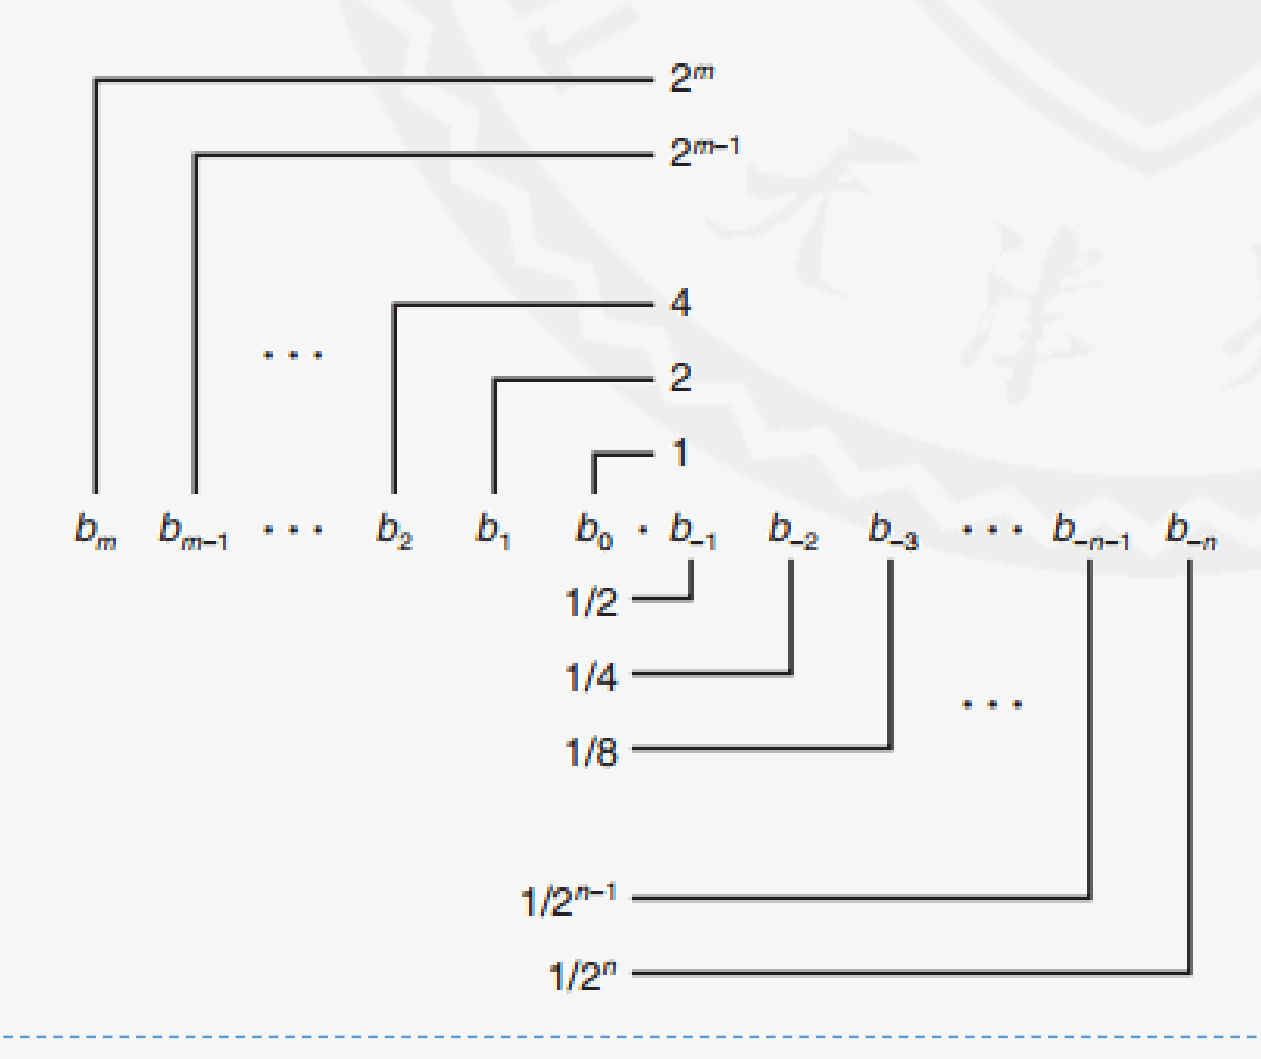
\includegraphics[width=6cm]{figures/1.png}
    \caption{小数的二进制表示}
\end{figure}


并且,除以2可通过逻辑右移实现,乘以2可通过左移实现。像\(0.11111\cdots_{2}\)这样的数字十分接近但小于1,可表示为\(1.0-\varepsilon\)。同时,并非所有有理数都能精确地用有限位二进制小数表示,例如\(\frac{1}{3}=0.0101010101[01]\cdots_{2}\),只能精确表示\(\frac{x}{2^{k}}\)这种形式的数字。

\subsection{IEEE浮点数的表示}
浮点数的表示形式为\((-1)^{s}\times M\times2^{E}\),其中:
\begin{itemize}
    \item 符号位\(s\)决定了数字的正负。
    \item 尾数\(M\)通常在\([1.0,2.0)\)或\([0.0,1.0)\)。
    \item 阶码\(E\)是浮点数的权重,为2的\(E\)次幂。
\end{itemize}
\begin{figure}[H]
    \centering
    \captionsetup{skip=4pt}
    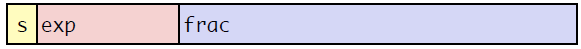
\includegraphics[width=10cm]{2.png}
    \caption{浮点数编码}
\end{figure}

编码方式为:最高位是符号位\(s\),\(\text{exp}\)编码后得到\(E\)(\(\text{exp}\neq E\)),\(\text{frac}\)编码后得到\(M\)(\(\text{frac}\neq M\))。

\subsubsection{几种精度的浮点数}

常见的浮点数精度有:
\begin{table}[h]
    \centering
    \begin{tabular}{|c|c|c|c|c|}
        \hline
        精度类型           & 总位数 & 符号位 & \(\text{exp}\)位数 & \(\text{frac}\)位数 \\
        \hline
        单精度            & 32位 & 1位  & 8位               & 23位               \\
        双精度            & 64位 & 1位  & 11位              & 52位               \\
        扩展精度(仅Intel支持) & 80位 & 1位  & 15位              & 63或64位            \\
        \hline
    \end{tabular}
    \caption{不同精度浮点数的位宽分布}
\end{table}

\subsubsection{规格化数}
当\(\text{exp}\neq000\cdots0\)且\(\text{exp}\neq111\cdots1\)时:
\begin{itemize}
    \item 尾数编码为包含一个隐式前置的1,即\(M = 1.x_1 x_2{\cdots}\),其中\(x_1x_2\cdots\)为\(\text{frac}\)域的各位的编码。
    \item 阶码为一个有偏置的指数,\(E=\text{Exp}-\text{Bias}\),\(\text{Exp}\)为\(\text{exp}\)域无符号数编码值,\(\text{bias}=2^{k - 1}-1\),\(k\)是\(\text{exp}\)的位宽。
    \item 例如,对于单精度浮点数,\(\text{bias}=127\)(\(\text{Exp}:1\cdots254\),\(E:-126\cdots127\));双精度浮点数,\(\text{bias}=1023\)(\(\text{Exp}:1\cdots2046\),\(E:-1022\cdots1023\))。隐式前置的整数1始终存在,因此在\(\text{frac}\)中不需要包含。
\end{itemize}
以\(\text{float }f = 15213.0\)为例:
\begin{align*}
    f=15213_{10}      & =1101101101101000000000_{2}           \\
                      & =1.1101101101101101_{2}\times2^{13}   \\
    \text{尾数 }\quad M & =1.\textbf{1101101101101101}_{2}      \\
    \text{frac}       & =\textbf{1101101101101} 000000000_{2} \\
    \text{阶码 }\quad E & =13,                                  \\
    \text{Bias}       & =2^{k-1}-1=127\quad(k=8),             \\
    \text{Exp}        & =140 = 10001100_{2}
\end{align*}
结果为\(0\quad10001100  \quad11011011011010000000000\)。

\subsubsection{非规格化数}
当\(\text{exp}=000\cdots0\)时:
\begin{itemize}
    \item 阶码\(E=-\text{Bias}+1\)(而不是\(E = 0-\text{Bias}\))。
    \item 尾数编码为包含一个隐式前置的0,即\(M = 0.x_1x_2\cdots\)。
    \item 当\(\text{exp}=000\cdots0\),且\(\text{frac}=000\cdots0\)时,表示0,要注意\(+0\)和\(-0\)的区别。
    \item 当\(\text{exp}=000\cdots0\),且\(\text{frac}\neq000\cdots0\)时,表示非常接近于0.0的数字,这些数字是等间距的。
\end{itemize}

\subsubsection{特殊值}
当\(\text{exp}=111\cdots1\)时:
\begin{itemize}
    \item 当\(\text{exp}=111\cdots1\)且\(\text{frac}=000\cdots0\)时,表示无穷\(\infty\),意味着运算出现了溢出,有正向溢出和负向溢出,例如\(1.0/0.0=-1.0/-0.0=+\infty\),\(1.0/-0.0=-\infty\)。
    \item 当\(\text{exp}=111\cdots1\)且\(\text{frac}\neq000\cdots0\)时,表示不是一个数字(NaN),表示数值无法确定,例如\(-1,\infty-\infty,\infty\times0\)。
\end{itemize}

\subsubsection{IEEE编码的特殊属性}
\begin{enumerate}
    \item 浮点数0和整数0编码相同,所有位都为0
    \item 几乎可以用无符号整数比较的方法实现浮点数的比较运算,但首先要比较符号位,同时要考虑\(-0 = 0\)和NaN的问题(NaN比其他值都大)
\end{enumerate}

\subsubsection{需要关注的数字}
不同类型的浮点数有一些特殊的数字:
\begin{table}[h]
    \centering
    \begin{tabular}{|c|c|c|c|c|c|}
        \hline
        描述      & \(\text{exp}\) & \(\text{frac}\) & 单精度值(十进制)                         & 双精度值(十进制)                          \\
        \hline
        零       & \(00\cdots00\) & \(0\cdots00\)   & 0.0                               & 0.0                                \\
        最小非规格化数 & \(00\cdots00\) & \(0\cdots01\)   & \(2^{-23}\times2^{-126}\)         & \(2^{-52}\times2^{-1022}\)         \\
        最大非规格化数 & \(00\cdots00\) & \(1\cdots11\)   & \((1-\varepsilon)\times2^{-126}\) & \((1-\varepsilon)\times2^{-1022}\) \\
        最小规格化数  & \(00\cdots01\) & \(0\cdots00\)   & \(1\times2^{-126}\)               & \(1\times2^{-1022}\)               \\
        一       & \(01\cdots11\) & \(0\cdots00\)   & 1.0                               & 1.0                                \\
        最大规格化数  & \(11\cdots10\) & \(1\cdots11\)   & \((2-\varepsilon)\times2^{127}\)  & \((2-\varepsilon)\times2^{1023}\)  \\
        \hline
    \end{tabular}
    \caption{不同精度浮点数的特殊值}
\end{table}

\subsubsection{举例:一个微型的浮点数编码系统}
以8位浮点数编码为例,最高位为符号位,接下来是4位\(\text{exp}\),偏置\(\text{Bias}\)为7,最后3位是\(\text{frac}\),与IEEE规范具有相同的形式,有规格化数、非规格化数,以及0、NaN和无穷的编码。
\begin{table}[h]
    \centering
    \begin{tabular}{|c|c|c|c|c|}
        \hline
        \(s\)  & \(\text{exp}\) & \(\text{frac}\) & \(E\)   & 值                                                     \\
        \hline
        0      & 0000           & 000             & -6      & 0                                                     \\
        0      & 0000           & 001             & -6      & \(\frac{1}{8}\times\frac{1}{64}=\frac{1}{512}\)(最接近0) \\
        \vdots & \vdots         & \vdots          & \vdots  & \vdots                                                \\
        0      & 1111           & 000             & \(n/a\) & inf                                                   \\
        \hline
    \end{tabular}
    \caption{8位浮点数编码示例}
\end{table}

\subsubsection{总结}
单精度浮点数可分为以下几类:
\begin{enumerate}
    \item 规格化数:\(\text{exp}\neq0000000\)且\(\text{exp}\neq11111111\)。
    \item 非规格化数:\(\text{exp}=00000000\),\(\text{frac}\neq0000000\)。
    \item 无穷:\(\text{exp}=11111111\),\(\text{frac}=00000000\)。
    \item NaN:\(\text{exp}=11111111\),\(\text{frac}\neq00000000\)。
\end{enumerate}




\subsection{几种舍入模式}
常见的舍入模式有:
\begin{enumerate}
    \item 向下舍入:舍入结果接近但不会大于实际结果。
    \item 向上舍入:舍入结果接近但不会小于实际结果。
    \item 向0舍入:舍入结果向0的方向靠近,如果为正数,舍入结果不大于实际结果;如果为负数,舍入结果不小于实际结果。
    \item 向偶数舍入:浮点数运算默认的舍入模式,其他的舍入模式都会统计偏差,一组正数的总和将始终被高估或低估。
\end{enumerate}
向偶数舍入适用于舍入至小数点后任何位置,当数字正好处在四舍五入的中间时,向最低位为偶数的方向舍入。例如:

\begin{table}[H]
    \captionsetup{skip=4pt}
    \centering
    \setlength{\arrayrulewidth}{1pt}
    \begin{tabular}{ccc}
        \hline
        \makebox[0.2\textwidth][c]{值} & \makebox[0.2\textwidth][c]{结果} & \makebox[0.4\textwidth][c]{说明} \\
        \noalign{\global\setlength{\arrayrulewidth}{0.5pt}}
        \hline
        1.2349999                     & 1.23                           & 比中间值小,四舍                       \\
        1.2350001                     & 1.24                           & 比中间值大,五入                       \\
        1.2350000                     & 1.24                           & 中间,向上舍入(偶数方向)                  \\
        1.2450000                     & 1.24                           & 中间,向下舍入(偶数方向)                  \\
        \noalign{\global\setlength{\arrayrulewidth}{1pt}}
        \hline
    \end{tabular}
    \caption{向偶数舍入示例}
\end{table}

在二进制数中,偶数方向意味着舍入后最后一位为0,中间意味着待舍入的部分为\(100\cdots_{2}\)。

\subsection{浮点数运算}
浮点数运算的基本思想是先计算出精确的值,然后将结果调整至目标的精度。如果阶码值过大,可能会导致溢出,可能会进行舍入以满足尾数的位宽。例如:
\begin{align*}
    x+^{f}y      & =\text{Round}(x + y)     \\
    x\times^{f}y & =\text{Round}(x\times y)
\end{align*}

\subsubsection{浮点数乘法}
对于浮点数\((-1)^{s_1}M_1 2^{E_1}\times(-1)^{s_2}M_2 2^{E_2}\):
\begin{itemize}
    \item 精确结果:\(M_1\times M_2\),阶码\(E = E_1 + E_2\),符号位\(s = s_1^{s_2}\)。
    \item 修正:如果\(M\geq2\),右移\(M\),并增大\(E\)的值;如果\(E\)超出范围,发生溢出;对\(M\)进行舍入以满足\(\text{frac}\)的位宽精度要求。在实际实现中,尾数相乘的细节较为繁琐。
\end{itemize}

\subsubsection{浮点数加法}
对于浮点数\((-1)^{s_1}M_1 2^{E_1}+(-1)^{s_2}M_2 2^{E_2}\)(假设\(E_1>E_2\)):
\begin{itemize}
    \item 精确结果:\((-1)^{s}M_2^{E}\),其中符号位\(s\)和尾数\(M\)是有符号数对齐后相加的结果,阶码\(E = E_2\)。
    \item 修正:如果\(M\geq2\),右移\(M\),并增大\(E\)的值;如果\(M<1\),左移\(M\) \(k\)位,然后\(E\)减去\(k\);如果\(E\)超出范围,发生溢出;对\(M\)进行舍入以满足\(\text{frac}\)的位宽精度要求。
\end{itemize}

\subsection{C语言中的浮点数}
C语言标准确保支持两种精度的浮点数,即float(单精度)和double(双精度)。在进行类型转换时:
\begin{itemize}
    \item double/float转int:截断尾数部分,向0舍入。标准中未定义越界和NaN的情况,通常设置为\(T_{Min}\)和\(T_{Max}\)。
    \item int转double:只要int的位宽小于等于53位,就能精确转换。
    \item int转float:会根据舍入模式进行舍入。
\end{itemize}

以下是一些C语言中浮点数操作的示例(假设d和f分别是float和double且不是NaN和无穷):

\begin{table}[H]
    \captionsetup{skip=4pt}
    \centering
    \setlength{\arrayrulewidth}{1pt}
    \begin{tabular}{cc}
        \hline
        \makebox[0.4\textwidth][c]{表达式}                      & \makebox[0.4\textwidth][c]{结果} \\
        \noalign{\global\setlength{\arrayrulewidth}{0.5pt}}
        \hline
        \lstinline[style=cstyle]{x == (int)(float) x}        & 否:有效数字为24位                     \\
        \lstinline[style=cstyle]{x == (int)(double) x}       & 是:有效数字为53位                     \\
        \lstinline[style=cstyle]{f == (float)(double) f}     & 是:提高精度                         \\
        \lstinline[style=cstyle]{d == ( float ) d}           & 否:丢失精度                         \\
        \lstinline[style=cstyle]{f == -(-f)}                 & 是:仅改变符号位                       \\
        \lstinline[style=cstyle]{2/3 == 2/3.0}               & 否:\(2/3 == 0\)                 \\
        \lstinline[style=cstyle]{if(d < 0.0)  ((d*2) < 0.0)} & 是                              \\
        \lstinline[style=cstyle]{d * d >= 0.0}               & 是                              \\
        \lstinline[style=cstyle]{(d + f) - d == f}           & 否:不满足结合律                       \\
        \noalign{\global\setlength{\arrayrulewidth}{1pt}}
        \hline
    \end{tabular}
    \caption{C语言中浮点数操作示例结果}
\end{table}

在浮点数运算中,存在精度和准确度的问题。例如\(0.1 + 0.1 + 0.1 + 0.1 + 0.1 + 0.1 + 0.1 + 0.1 + 0.1+ 0.1 \neq1\),但\(0.2+0.2+0.2+0.2+0.2=1\)。在使用浮点数进行比较时,如\lstinline[style=cstyle]{if (d1 - d2 == 0)},需要谨慎处理,因为浮点数的精度限制可能导致结果不准确。在进行浮点数运算时,要充分考虑精度损失对计算结果的影响。

\section{程序的机器级表示:基础知识}
\subsection{Intel处理器体系结构的历史}

\subsubsection{复杂指令集计算机(CISC)}
Intel x86系列属于复杂指令集计算机,其指令多、格式复杂。理论上 CISC 的性能较难与精简指令集计算机(RISC)相比。在低功耗场景下,其速度会受到影响。


\subsubsection{摩尔定律}
摩尔定律指出,单位面积上可以容纳的晶体管数量几乎每两年增加一倍


% \subsubsection{Intel 64位体系结构发展的历史}
% 2001年,Intel试图从IA32转变为IA64(安腾),但性能令人失望。2003年,AMD提出x86 - 64位体系结构(现称为AMD64)。2004年,Intel提出EM64T体系结构,实现对IA32的64位扩展,几乎与x86 - 64相同。2019年,英特尔宣布放弃IA64架构,目前除低端x86处理器外,其他处理器均支持x86 - 64,但仍有许多程序在32位模式下运行。
\subsection{C语言,汇编语言和机器语言}
\subsubsection{定义}
\begin{enumerate}
    \item 体系结构(指令集体系结构,ISA):编写汇编代码时需要理解的处理器设计部分,如指令集规范、寄存器组织等。
    \item 微体系结构:体系结构的具体实现,例如高速缓存大小、核心频率等。
    \item 机器语言是处理器可以直接执行的字节级程序,汇编语言是文本形式的机器语言。
\end{enumerate}
常见的指令集体系结构有Intel的x86、IA32、Itanium、x86 - 64,以及ARM(用于几乎所有移动电话)。

\subsubsection{程序员可见的状态}
\begin{enumerate}
    \item 程序计数器(PC,在x86 - 64中称为RIP),存储下一条要执行指令的地址
    \item 条件码,存储最近一次算术逻辑运算的状态信息,用于条件分支
    \item 存储器,基于字节寻址,存储程序、用户数据和栈数据
    \item 寄存器文件,频繁用于存储程序数据
\end{enumerate}

\begin{figure}[H]
    \centering
    \captionsetup{skip=4pt}
    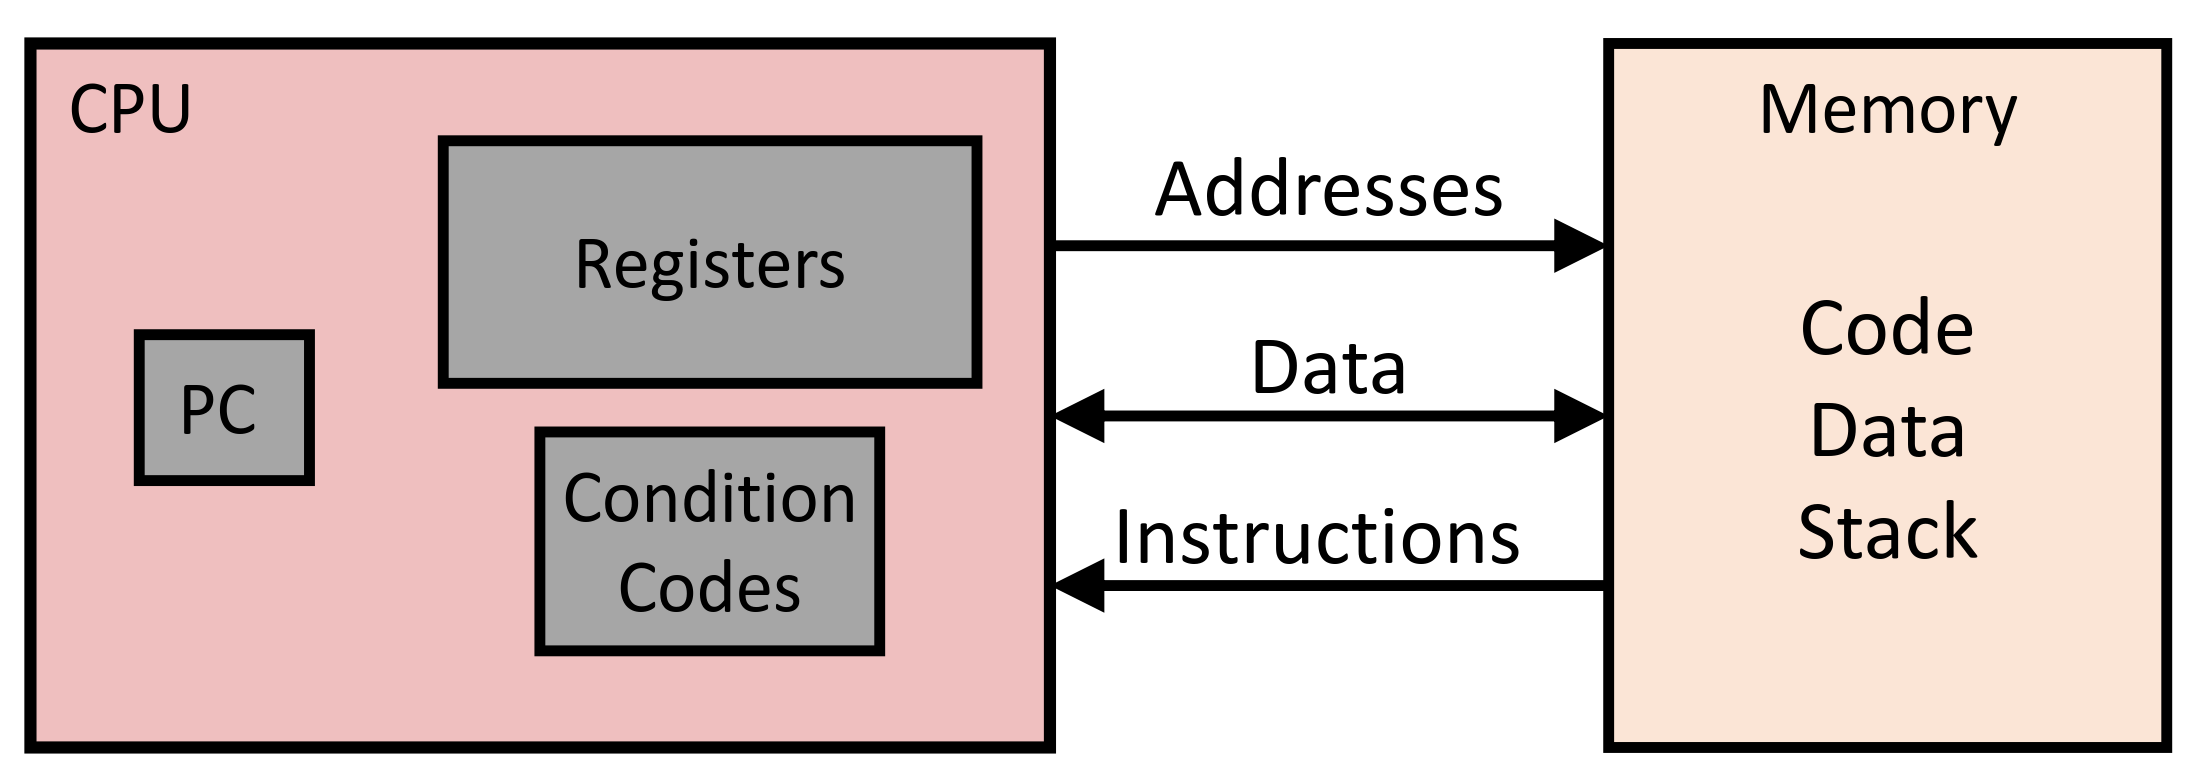
\includegraphics[width=10cm]{4.png}
    \caption{}
\end{figure}


\subsubsection{汇编语言的数据类型}
\begin{enumerate}
    \item 整数:1、2、4或8字节
    \item 地址:无类型的指针
    \item 浮点数:4、8或10字节
    \item 代码:指令的字节序列编码
\end{enumerate}
与C语言不同,汇编语言没有聚合类型,数组或结构体在汇编语言中表现为在内存中连续分配的字节。

\subsubsection{汇编语言的操作}
汇编语言可以对寄存器或存储器数据执行算术/逻辑运算,在寄存器和存储器间传输数据(包括将数据从存储器加载至寄存器以及将寄存器的数据存储至存储器),还能进行转移控制,如无条件跳转至/从过程、条件分支等。

% \subsubsection{链接器}
% 链接器将 `.s` 文件翻译为 `.o` 文件,对每条指令进行二进制编码,生成几乎完整的可执行代码,但缺少不同文件的链接信息。链接器实现了不同文件间的引用,并与静态链接库结合(例如代码中的 `malloc`、`printf` 等),某些库需要动态链接,链接在程序开始执行时进行。

\subsubsection{举例:机器指令}
对于C语言代码 \mintinline{c}{*dest = t;},对应的汇编代码 \mintinline{asm}{movq %rax, (%rbx)},将8字节数据移动至存储器。其操作数 t 存储在寄存器 \mintinline{asm}{%rax}中,dest 存储在寄存器  \mintinline{asm}{%rbx} 中,*dest 表示内存地址  \mintinline{asm}{M[%rbx]}。对应目标码(机器指令)为\mintinline{asm}{0x40059e: 48 89 03},该指令为3字节,存储于地址0x40059e。

\subsubsection{反汇编}
反汇编器是探索目标码的有用工具,它可以分析指令的编码序列,根据目标码重新生成汇编代码,并且可以对任何可执行程序文件和 \mintinline{c}{.o} 文件进行反汇编。例如使用 \mintinline{bash}{objdump –d sum} 对 sum 文件进行反汇编,或者在 gdb 调试器中使用 \mintinline{bash}{gdb sum} 以及 \mintinline{bash}{disassemble sumstore} 反汇编 sumstore 函数。反汇编程序会分析字节并重构为汇编代码。

\section{程序的机器级表示:基本操作}
\subsection{x86寄存器}
\subsubsection{x86 - 64寄存器}
x86 - 64架构下,每个寄存器的低4/2/1字节都有唯一的标识。其包含多个寄存器,如 \mintinline{asm}{\%rax}、\mintinline{asm}{\%rbx}、\mintinline{asm}{\%rcx} 等。其中\mintinline{asm}{\%rsp}有特殊用途,一般不在汇编里使用。寄存器具体如下:
\begin{table}[H]
    \captionsetup{skip=4pt}
    \centering
    \setlength{\arrayrulewidth}{1pt}
    \begin{tabular}{cccc}
        \hline
        63 - 31位 & 31 - 15位 & 15 - 7位 & 7 - 0位 \\
        \hline
        \mintinline{asm}{%rax} & \mintinline{asm}{%eax}  & \mintinline{asm}{%ax}   & \mintinline{asm}{%al}   \\
        \mintinline{asm}{%rbx} & \mintinline{asm}{%ebx}  & \mintinline{asm}{%bx}   & \mintinline{asm}{%bl}   \\
        \mintinline{asm}{%rcx} & \mintinline{asm}{%ecx}  & \mintinline{asm}{%cx}   & \mintinline{asm}{%cl}   \\
        \mintinline{asm}{%rdx} & \mintinline{asm}{%edx}  & \mintinline{asm}{%dx}   & \mintinline{asm}{%dl}   \\
        \mintinline{asm}{%rsi} & \mintinline{asm}{%esi}  & \mintinline{asm}{%si}   & \mintinline{asm}{%sil}  \\
        \mintinline{asm}{%rdi} & \mintinline{asm}{%edi}  & \mintinline{asm}{%di}   & \mintinline{asm}{%dil}  \\
        \mintinline{asm}{%rbp} & \mintinline{asm}{%ebp}  & \mintinline{asm}{%bp}   & \mintinline{asm}{%bp}   \\
        \mintinline{asm}{%rsp} & \mintinline{asm}{%esp}  & \mintinline{asm}{%sp}   & \mintinline{asm}{%spl}  \\
        \mintinline{asm}{%r8}  & \mintinline{asm}{%r8d}  & \mintinline{asm}{%r8w}  & \mintinline{asm}{%r8b}  \\
        \mintinline{asm}{%r9}  & \mintinline{asm}{%r9d}  & \mintinline{asm}{%r9w}  & \mintinline{asm}{%r9b}  \\
        \mintinline{asm}{%r10} & \mintinline{asm}{%r10d} & \mintinline{asm}{%r10w} & \mintinline{asm}{%r10b} \\
        \mintinline{asm}{%r11} & \mintinline{asm}{%r11d} & \mintinline{asm}{%r11w} & \mintinline{asm}{%r11b} \\
        \mintinline{asm}{%r12} & \mintinline{asm}{%r12d} & \mintinline{asm}{%r12w} & \mintinline{asm}{%r12b} \\
        \mintinline{asm}{%r13} & \mintinline{asm}{%r13d} & \mintinline{asm}{%r13w} & \mintinline{asm}{%r13b} \\
        \mintinline{asm}{%r14} & \mintinline{asm}{%r14d} & \mintinline{asm}{%r14w} & \mintinline{asm}{%r14b} \\
        \mintinline{asm}{%r15} & \mintinline{asm}{%r15d} & \mintinline{asm}{%r15w} & \mintinline{asm}{%r15b} \\
        \hline
    \end{tabular}
    \caption{x86 - 64寄存器各部分标识}
\end{table}
\subsubsection{IA32 (x86 - 32)寄存器}
IA32(x86 - 32)架构下的寄存器有 \mintinline{asm}{%eax}、\mintinline{asm}{%ecx}、\mintinline{asm}{%edx} 等,其各部分标识如下:
\begin{table}[H]
    \captionsetup{skip=4pt}
    \centering
    \setlength{\arrayrulewidth}{1pt}
    \begin{tabular}{cccc}
        \hline
        31 - 15位 & 15 - 7位 & 7 - 0位 \\
        \hline
        \mintinline{asm}{%eax} & \mintinline{asm}{%ax} & \mintinline{asm}{%al} \\
        \mintinline{asm}{%ecx} & \mintinline{asm}{%cx} & \mintinline{asm}{%cl} \\
        \mintinline{asm}{%edx} & \mintinline{asm}{%dx} & \mintinline{asm}{%dl} \\
        \mintinline{asm}{%ebx} & \mintinline{asm}{%bx} & \mintinline{asm}{%bl} \\
        \mintinline{asm}{%esi} & \mintinline{asm}{%si} & -                      \\
        \mintinline{asm}{%edi} & \mintinline{asm}{%di} & -                      \\
        \mintinline{asm}{%esp} & \mintinline{asm}{%sp} & -                      \\
        \mintinline{asm}{%ebp} & \mintinline{asm}{%bp} & -                      \\
        \hline
    \end{tabular}
    \caption{IA32 (x86 - 32)寄存器各部分标识}
\end{table}
\subsection{数据移动指令}
\subsubsection{汇编语言格式}
汇编语言格式为 \mintinline{asm}{[label :] [opcode] [operand 1] [, operand 2]},即\[\text{标号:} \text{操作码} \text{操作数}1 [\text{,操作数}2]\]。例如,在ATT assembly中:
\begin{minted}{asm}
l1: movq $5, %rax
addq $-16, (%rax)
\end{minted}
在Intel assembly中:
\begin{minted}{asm}
l1: mov rax, 5
add QWORD PTR[rax], -16
\end{minted}
\subsubsection{操作数类型}
操作数类型包含:
\begin{enumerate}[label=\arabic*.]
    \item \textbf{立即数}:整数常量,如 \mintinline{asm}{\$0x400}、\mintinline{asm}{\$-533} ,和C语言中的常数类似,但需要加前缀 \mintinline{asm}{\$},其被编码为1、2、4或8个字节。
    \item \textbf{寄存器}:十六个整数寄存器之一,如 \mintinline{asm}{\%rax}、\mintinline{asm}{\%r13} 。其中 \mintinline{asm}{\%rsp} 有特殊用途,通常不使用,其他寄存器在一些特殊的指令中也会有特殊用途。
    \item \textbf{存储器}:指向的内存中8个连续字节,由寄存器给出地址,例如 \mintinline{asm}{(\%rax)} ,还有很多其他的“寻址模式”。
\end{enumerate}
\subsubsection{movq指令操作数的几种组合}
\begin{table}[H]
    \captionsetup{skip=4pt}
    \centering
    \setlength{\arrayrulewidth}{1pt}
    \begin{tabular}{cccc}
        \hline
        源操作数Src & 目标操作数Dest & 示例                                     & 等价C语言C Analog                  \\
        \hline
        立即数     & 寄存器       & \mintinline{asm}{movq \$0x4, \%rax}    & \mintinline{c}{temp = 0x4;}    \\
        立即数     & 存储器       & \mintinline{asm}{movq \$-147, (\%rax)} & \mintinline{c}{*p = -147;}     \\
        寄存器     & 寄存器       & \mintinline{asm}{movq \%rax, \%rdx}    & \mintinline{c}{temp2 = temp1;} \\
        寄存器     & 存储器       & \mintinline{asm}{movq \%rax, (\%rdx)}  & \mintinline{c}{*p = temp;}     \\
        存储器     & 寄存器       & \mintinline{asm}{movq (\%rax), \%rdx}  & \mintinline{c}{temp = *p;}     \\
        \hline
    \end{tabular}
    \caption{movq指令操作数组合及等价C语言表达}
\end{table}
\subsubsection{数据格式}
不同C语言类型声明对应不同的数据类型、操作码后缀和大小,具体如下:
\begin{table}[H]
    \captionsetup{skip=4pt}
    \centering
    \setlength{\arrayrulewidth}{1pt}
    \begin{tabular}{cccc}
        \hline
        C语言类型声明                & 数据类型             & 操作码后缀 & 大小(bytes) \\
        \hline
        \mintinline{c}{char}   & Byte             & b     & 1         \\
        \mintinline{c}{short}  & Word             & w     & 2         \\
        \mintinline{c}{int}    & Double Word      & l     & 4         \\
        \mintinline{c}{long}   & Quad Word        & q     & 8         \\
        \mintinline{c}{char *} & Quad Word        & q     & 8         \\
        \mintinline{c}{float}  & Single precision & s     & 4         \\
        \mintinline{c}{Double} & Double precision & l     & 8         \\
        \hline
    \end{tabular}
    \caption{C语言类型与数据格式对应关系}
\end{table}
\subsubsection{几种简单的存储器寻址模式}
\begin{enumerate}[label=\arabic*.]
    \item \textbf{间接寻址}: \mintinline{asm}{(R)} 表示 \mintinline{asm}{Mem[Reg[R]]} ,寄存器 \mintinline{asm}{R} 指向了存储器的地址,和C语言中的指针作用相同,例如 \mintinline{asm}{movq (\%rcx),\%rax} 。
    \item \textbf{基地址 + 偏移量寻址}: \mintinline{asm}{D(R)} 表示 \mintinline{asm}{Mem[Reg[R]+D]} ,寄存器 \mintinline{asm}{R} 指定了存储器区域的开始位置,常数 \mintinline{asm}{D} 是偏移量,例如 \mintinline{asm}{movq 8(\%rbp),\%rdx} 。
\end{enumerate}
\subsubsection{举例:简单寻址模式(swap函数)}
以 \mintinline{c}{swap} 函数为例:
\begin{minted}{c}
void swap(long *xp, long *yp) 
{
    long t0 = *xp;
    long t1 = *yp; 
    *xp = t1; 
    *yp = t0;
}
\end{minted}
其汇编代码如下:
\begin{minted}{asm}
swap:
movq (%rdi), %rax # t0 = *xp
movq (%rsi), %rdx # t1 = *yp
movq %rdx, (%rdi) # *xp = t1
movq %rax, (%rsi) # *yp = t0
ret
\end{minted}
在该函数中, \mintinline{asm}{\%rdi} 存放 \mintinline{c}{xp} 的值, \mintinline{asm}{%rsi} 存放 \mintinline{c}{yp} 的值, \mintinline{asm}{%rax} 用于存放 \mintinline{c}{t0} , \mintinline{asm}{%rdx} 用于存放 \mintinline{c}{t1} 。通过逐步执行这些指令,实现两个指针所指向的值的交换。
\subsubsection{完整的存储器寻址模式}
最通用的形式为 \mintinline{asm}{D(R_{b}, R_{i}, S)} 表示 \mintinline{asm}{Mem[Reg[R_{b}]+S * Reg[R_{i}]+D]} ,其中:
\begin{enumerate}[label=\arabic*.]
    \item \mintinline{asm}{D}:常数偏移量,可以为1、2、4或8字节整数。
    \item \mintinline{asm}{R_{b}}:基地址寄存器,是16个寄存器之一。
    \item \mintinline{asm}{R_{i}}:变址寄存器,除 \mintinline{asm}{\%rsp} 外的其他寄存器。
    \item \mintinline{asm}{S}:比例因子,可以为1、2、4或8。
\end{enumerate}
还有一些特殊形式,如 \mintinline{asm}{(R_{b}, R_{i})} 表示 \mintinline{asm}{Mem[Reg[R_{b}] + Reg[R_{i}]]} , \mintinline{asm}{D(R_{b}, R_{i})} 表示 \mintinline{asm}{Mem[Reg[R_{b}]+Reg[R_{i}]+D]} , \mintinline{asm}{(R_{b}, R_{i}, S)} 表示 \mintinline{asm}{Mem[Reg[R_{b}]+S * Reg[R_{i}]]} 。
\subsubsection{小练习:地址计算}
假设 \mintinline{asm}{\%rdx = 0xf000}, \mintinline{asm}{\%rcx = 0x0100} ,不同地址表达式的计算结果如下:
\begin{table}[H]
    \captionsetup{skip=4pt}
    \centering
    \setlength{\arrayrulewidth}{1pt}
    \begin{tabular}{ccc}
        \hline
        表达式 & 地址计算 & 地址 \\
        \hline
        \mintinline{asm}{0x8(%rdx)}      & \mintinline{asm}{0xf000 + 0x8}     & \mintinline{asm}{0xf008}  \\
        \mintinline{asm}{(%rdx,%rcx)}   & \mintinline{asm}{0xf000 + 0x100}   & \mintinline{asm}{0xf100}  \\
        \mintinline{asm}{(%rdx,%rcx,4)} & \mintinline{asm}{0xf000 + 4*0x100} & \mintinline{asm}{0xf400}  \\
        \mintinline{asm}{0x80(,%rdx,2)}  & \mintinline{asm}{2*0xf000 + 0x80}  & \mintinline{asm}{0x1e080} \\
        \hline
    \end{tabular}
    \caption{不同地址表达式的计算结果}
\end{table}
\subsection{算术、逻辑运算指令}
\subsubsection{地址计算指令(leaq)}
\mintinline{asm}{leaq} 指令格式为 \mintinline{asm}{leaq Src, Dst},其中 \mintinline{asm}{Src} 是寻址模式表达式,该指令将表达式计算的地址写入 \mintinline{asm}{Dst} 。其用途包括计算地址(计算过程中不需要引用存储器),例如 \mintinline{c}{p=& x[i]} ;还可计算模式为 \mintinline{c}{x + k*y}( \mintinline{c}{k = 1, 2, 4} 或8)的表达式。例如,对于函数:
\begin{minted}{c}
long m12(long x)
{
    return x*12;
}
\end{minted}
编译后的汇编指令为:
\begin{minted}{asm}
leaq (%rdi,%rdi,2), %rax # t <- x+x*2
salq $2, %rax # return t<<2
\end{minted}
\subsubsection{一些算术运算指令(两操作数指令)}
两操作数指令(双目运算)的格式及计算方式如下:
\begin{table}[H]
    \captionsetup{skip=4pt}
    \centering
    \setlength{\arrayrulewidth}{1pt}
    \begin{tabular}{ccc}
        \hline
        格式                                & 计算                                   & 说明                            \\
        \hline
        \mintinline{asm}{addq Src, Dest}  & \mintinline{asm}{Dest = Dest + Src}  & -                             \\
        \mintinline{asm}{subq Src, Dest}  & \mintinline{asm}{Dest = Dest - Src}  & -                             \\
        \mintinline{asm}{imulq Src, Dest} & \mintinline{asm}{Dest = Dest * Src}  & -                             \\
        \mintinline{asm}{salq Src, Dest}  & \mintinline{asm}{Dest = Dest << Src} & 也叫 \mintinline{asm}{shlq}     \\
        \mintinline{asm}{sarq Src, Dest}  & \mintinline{asm}{Dest = Dest >> Src} & 算术右移                          \\
        \mintinline{asm}{shrq Src, Dest}  & \mintinline{asm}{Dest = Dest >> Src} & 逻辑右移                          \\
        \mintinline{asm}{xorq Src, Dest}  & \mintinline{asm}{Dest = Dest ^ Src}  & -                             \\
        \mintinline{asm}{andq Src, Dest}  & \mintinline{asm}{Dest = Dest         & Src}                      & - \\
        \mintinline{asm}{orq Src, Dest}   & \mintinline{asm}{Dest = Dest | Src}  & -                             \\
        \hline
    \end{tabular}
    \caption{两操作数算术运算指令}
\end{table}
需要注意操作数的顺序,并且有符号数和无符号数指令没有区别。
\subsubsection{一些算术运算指令(单操作数指令)}
单操作数指令(单目运算)的格式及计算方式如下:
\begin{table}[H]
    \captionsetup{skip=4pt}
    \centering
    \setlength{\arrayrulewidth}{1pt}
    \begin{tabular}{cc}
        \hline
        格式                          & 计算                                \\
        \hline
        \mintinline{asm}{incq Dest} & \mintinline{asm}{Dest = Dest + 1} \\
        \mintinline{asm}{decq Dest} & \mintinline{asm}{Dest = Dest - 1} \\
        \mintinline{asm}{negq Dest} & \mintinline{asm}{Dest = - Dest}   \\
        \mintinline{asm}{notq Dest} & \mintinline{asm}{Dest = ~Dest}    \\
        \hline
    \end{tabular}
    \caption{单操作数算术运算指令}
\end{table}
更多指令可查阅教材。
\subsubsection{需要关注的指令及举例:算术运算}
需要关注的指令有 \mintinline{asm}{leaq}(地址计算)、 \mintinline{asm}{salq}(左移)、 \mintinline{asm}{imulq}(乘法)等。以函数:
\begin{minted}{c}
long arith(long x, long y, long z)
{
    long t1 = x+y;
    long t2 = z+t1;
    long t3 = x+4;
    long t4 = y * 48;
    long t5 = t3 + t4;
    long rval = t2 * t5;
    return rval;
}
\end{minted}
其汇编代码为:
\begin{minted}{asm}
arith:
addq %rsi, %rdi       # t1 = x + y
addq %rdi, %rdx       # t2 = z + t1
leaq 4(%rdi), %rax    # t3 = x + 4
leaq (%rsi,%rsi,2), %rcx  # t4a = y + 2*y
salq $4, %rcx         # t4 = t4a << 4
addq %rcx, %rax       # t5 = t3 + t4
imulq %rax, %rdx      # rval = t2 * t5
movq %rdx, %rax       # return rval
ret
\end{minted}
此函数的汇编代码通过一系列指令实现了函数中各变量的计算。首先将 \mintinline{asm}{x} 和 \mintinline{asm}{y} 相加得到 \mintinline{asm}{t1},再把 \mintinline{asm}{t1} 与 \mintinline{asm}{z} 相加得到 \mintinline{asm}{t2}。对于 \mintinline{asm}{t3},使用 \mintinline{asm}{leaq} 指令计算 \mintinline{asm}{x + 4}。计算 \mintinline{asm}{t4} 时,先通过 \mintinline{asm}{leaq} 计算 \mintinline{asm}{y + 2*y} 得到 \mintinline{asm}{t4a},再左移4位得到 \mintinline{asm}{t4}。然后将 \mintinline{asm}{t3} 和 \mintinline{asm}{t4} 相加得到 \mintinline{asm}{t5},最后将 \mintinline{asm}{t2} 和 \mintinline{asm}{t5} 相乘得到结果 \mintinline{asm}{rval} 并返回。

\subsection{控制转移指令}
\subsubsection{条件码寄存器}
CPU中有一组单个位的条件码寄存器,常用的有:
\begin{itemize}
    \item \mintinline{asm}{CF}(进位标志):无符号运算产生进位时设置。
    \item \mintinline{asm}{ZF}(零标志):结果为零时设置。
    \item \mintinline{asm}{SF}(符号标志):结果为负时设置。
    \item \mintinline{asm}{OF}(溢出标志):有符号运算溢出时设置。
\end{itemize}
很多算术和逻辑指令都会设置这些条件码,例如 \mintinline{asm}{addq}、\mintinline{asm}{subq} 等。

\subsubsection{比较和测试指令}
比较指令 \mintinline{asm}{cmpq} 和测试指令 \mintinline{asm}{testq} 主要用于设置条件码,而不改变任何寄存器或内存的值。
\mintinline{asm}{cmpq Src2, Src1} 相当于计算 \mintinline{asm}{Src1 - Src2} 并设置条件码,例如:
\begin{minted}{asm}
cmpq %rdi, %rsi  # 设置条件码,基于 %rsi - %rdi
\end{minted}
\mintinline{asm}{testq Src2, Src1} 相当于计算 \mintinline{asm}{Src1 & Src2} 并设置条件码,例如:
\begin{minted}{asm}
testq %rdi, %rdi  # 判断 %rdi 是否为零
\end{minted}

\subsubsection{条件跳转指令}
条件跳转指令根据条件码的值来决定是否跳转。例如:
\begin{itemize}
    \item \mintinline{asm}{je}(等于跳转):当 \mintinline{asm}{ZF = 1} 时跳转。
    \item \mintinline{asm}{jne}(不等于跳转):当 \mintinline{asm}{ZF = 0} 时跳转。
    \item \mintinline{asm}{jg}(大于跳转):有符号比较中,当 \mintinline{asm}{SF = OF} 且 \mintinline{asm}{ZF = 0} 时跳转。
    \item \mintinline{asm}{jge}(大于等于跳转):有符号比较中,当 \mintinline{asm}{SF = OF} 时跳转。
    \item \mintinline{asm}{jl}(小于跳转):有符号比较中,当 \mintinline{asm}{SF != OF} 时跳转。
    \item \mintinline{asm}{jle}(小于等于跳转):有符号比较中,当 \mintinline{asm}{SF != OF} 或 \mintinline{asm}{ZF = 1} 时跳转。
    \item \mintinline{asm}{ja}(高于跳转):无符号比较中,当 \mintinline{asm}{CF = 0} 且 \mintinline{asm}{ZF = 0} 时跳转。
    \item \mintinline{asm}{jae}(高于等于跳转):无符号比较中,当 \mintinline{asm}{CF = 0} 时跳转。
    \item \mintinline{asm}{jb}(低于跳转):无符号比较中,当 \mintinline{asm}{CF = 1} 时跳转。
    \item \mintinline{asm}{jbe}(低于等于跳转):无符号比较中,当 \mintinline{asm}{CF = 1} 或 \mintinline{asm}{ZF = 1} 时跳转。
\end{itemize}
示例代码:
\begin{minted}{asm}
cmpq %rdi, %rsi
jg greater  # 如果 %rsi > %rdi 则跳转到 greater 标签处
# 不满足条件时执行的代码
jmp end
greater:
# 满足条件时执行的代码
end:
\end{minted}

\subsubsection{无条件跳转指令}
无条件跳转指令 \mintinline{asm}{jmp} 会直接跳转到指定的位置。可以是直接跳转(给出标签),也可以是间接跳转(通过寄存器或内存地址)。
直接跳转示例:
\begin{minted}{asm}
jmp target  # 跳转到 target 标签处
target:
# 跳转后的代码
\end{minted}
间接跳转示例:
\begin{minted}{asm}
jmp *%rax  # 跳转到 %rax 所指向的地址处
\end{minted}

\subsubsection{循环和分支结构的实现}
在汇编中,循环和分支结构通常通过条件码和跳转指令来实现。

\paragraph{while 循环示例}
C 语言的 while 循环:
\begin{minted}{c}
long fact_while(long n) {
    long result = 1;
    while (n > 1) {
        result *= n;
        n--;
    }
    return result;
}
\end{minted}
对应的汇编代码:
\begin{minted}{asm}
fact_while:
movl $1, %eax  # result = 1
cmpq $1, %rdi  # 比较 n 和 1
jle done       # 如果 n <= 1 则跳转到 done
loop:
imulq %rdi, %rax  # result *= n
subq $1, %rdi     # n--
cmpq $1, %rdi     # 比较 n 和 1
jg loop          # 如果 n > 1 则跳转到 loop
done:
movq %rax, %rdi  # 返回 result
ret
\end{minted}

\paragraph{if - else 分支示例}
C 语言的 if - else 语句:
\begin{minted}{c}
long absdiff(long x, long y) {
    if (x < y) {
        return y - x;
    } else {
        return x - y;
    }
}
\end{minted}
对应的汇编代码:
\begin{minted}{asm}
absdiff:
cmpq %rsi, %rdi  # 比较 x 和 y
jl less          # 如果 x < y 则跳转到 less
subq %rsi, %rdi  # x - y
movq %rdi, %rax  # 返回结果
ret
less:
subq %rdi, %rsi  # y - x
movq %rsi, %rax  # 返回结果
ret
\end{minted}

\subsection{过程调用和栈管理}
\subsubsection{栈的基本概念}
栈是一种后进先出(LIFO)的数据结构,在 x86 - 64 中,栈从高地址向低地址增长, \mintinline{asm}{\%rsp} 寄存器指向栈顶。栈主要用于存储局部变量、保存返回地址和寄存器状态等。

\subsubsection{过程调用指令}
\mintinline{asm}{call} 指令用于调用一个过程,它会将下一条指令的地址(返回地址)压入栈中,并跳转到被调用过程的起始地址。例如:
\begin{minted}{asm}
call proc  # 调用 proc 过程
# 调用返回后执行的代码
\end{minted}
\mintinline{asm}{ret} 指令用于从过程中返回,它会从栈中弹出返回地址,并跳转到该地址继续执行。

\subsubsection{栈帧结构}
每个过程在栈上都有一个栈帧(stack frame),栈帧包含局部变量、保存的寄存器值等。栈帧的底部由 \mintinline{asm}{\%rbp} 寄存器指向(基指针),栈帧的顶部由 \mintinline{asm}{\%rsp} 寄存器指向(栈指针)。

进入一个过程时,通常会保存当前的 \mintinline{asm}{\%rbp} 值,并将 \mintinline{asm}{\%rsp} 的值赋给 \mintinline{asm}{\%rbp},以建立新的栈帧。例如:
\begin{minted}{asm}
pushq %rbp    # 保存旧的 %rbp
movq %rsp, %rbp  # 建立新的栈帧
# 过程体代码
popq %rbp     # 恢复旧的 %rbp
ret           # 返回
\end{minted}

\subsubsection{参数传递}
在 x86 - 64 中,前六个整数或指针参数依次通过 \mintinline{asm}{\%rdi}、\mintinline{asm}{\%rsi}、\mintinline{asm}{\%rdx}、\mintinline{asm}{\%rcx}、\mintinline{asm}{\%r8}、\mintinline{asm}{\%r9} 寄存器传递,更多的参数则通过栈传递。返回值通常通过 \mintinline{asm}{\%rax} 寄存器返回。

例如,一个接收两个参数的函数:
\begin{minted}{c}
long add(long a, long b) {
    return a + b;
}
\end{minted}
调用该函数的汇编代码示例:
\begin{minted}{asm}
movq $3, %rdi  # 参数 a = 3
movq $5, %rsi  # 参数 b = 5
call add       # 调用 add 函数
# 返回值在 %rax 中
\end{minted}
\section{程序的机器级表示:控制}
\subsection{条件码}
\subsubsection{处理器状态与条件码概述}
在 x86 - 64 架构中,处理器状态包含多个部分,存储当前程序的执行信息
\begin{enumerate}
    \item 临时数据,\mintinline{asm}{%rax} 等
    \item 运行时栈的位置(栈顶),\mintinline{asm}{%rsp}
    \item 当前代码控制点的位置(即将要执行的指令地址),\mintinline{asm}{%rip}
    \item 条件码,包括CF、ZF、SF、OF
\end{enumerate}
条件码寄存器是简单的位寄存器,通过算术运算、比较指令和测试指令等进行设置。

\subsubsection{条件码含义}
\begin{enumerate}
    \item CF: 进位标志 (Carry Flag)。最近的操作使无符号数最高位产生了进位,可用来检查无符号操作的溢出
    \item ZF: 零标志 (Zero Flag)。最近的操作得出的结果为 0
    \item SF: 符号标志 (Sign Flag)。最近的操作得到的结果为负数
    \item OF: 溢出标志 (Overflow Flag)。最近的操作导致一个有符号数补码溢出
\end{enumerate}


\subsubsection{条件码的设置方式}
\begin{enumerate}
    \item \textbf{算术运算隐式设置}: \mintinline{asm}{addq Src, Dest},相当于$t =a + b$

          这类算术运算指令会隐式设置条件码。若运算时出现无符号数运算溢出,CF 被置位;若 \(t == 0\),ZF 被置位;若有符号数 \(t < 0\)(,SF 被置位;若有符号数运算出现溢出,即 \mintinline{c}{(a > 0 && b > 0 && t < 0) || (a < 0 && b < 0 && t >= 0)},OF 被置位。需要注意的是,\mintinline{asm}{\leaq} 指令不修改条件码。
    \item \textbf{比较指令显式设置}:\mintinline{asm}{cmpq Src2, Src1}(如 \mintinline{asm}{cmpq b,a} )

          指令类似于计算 \(a - b\),但不将结果写入目标寄存器,而是根据计算结果显式设置条件码。当运算时出现超出最高位的借位(用于无符号数比较),CF 被置位;若 \(a == b\),ZF 被置位;若 \((a - b)<0\)(看做有符号数),SF 被置位;若有符号数运算出现溢出,即 \mintinline{c}{(a > 0 && b < 0 && (a - b) < 0) || ( a < 0 && b > 0 && (a - b) > 0)} ,OF 被置位。
    \item \textbf{测试指令显式设置}:\mintinline{asm}{testq Src2, Src1}(如 \mintinline{asm}{testq b,a} )

          指令类似于计算 \(a \& b\),同样不将结果写入目标寄存器,而是根据 \(a \& b\) 的结果设置条件码。常用于对一个操作数的某几个位进行掩码检测,当 \(a \& b == 0\) 时,ZF 被置位;若 \((a \& b)<0\),SF 被置位。
\end{enumerate}

\subsubsection{读取条件码与 SetX 指令}
SetX 指令可根据条件码表达式将目标寄存器的最后一个字节修改为 0 或 1,且不会影响目标寄存器最高 7 个字节的值。常见的 SetX 指令如下:
\begin{table}[H]
    \captionsetup{skip=4pt}
    \centering
    \setlength{\arrayrulewidth}{1pt}
    \begin{tabular}{ccc}
        \hline
        SetX 指令                 & 条件                           & 描述                   \\
        \hline
        \mintinline{asm}{sete}  & \mintinline{asm}{ZF}         & 相等/为零                \\
        \mintinline{asm}{setne} & \mintinline{asm}{~ZF}        & 不相等/不为零              \\
        \mintinline{asm}{sets}  & \mintinline{asm}{SF}         & 负数                   \\
        \mintinline{asm}{setns} & \mintinline{asm}{~SF}        & 非负数                  \\
        \mintinline{asm}{setg}  & \mintinline{asm}{~(SF^OF)    & ~ZF}       & 大于(有符号) \\
        \mintinline{asm}{setge} & \mintinline{asm}{~(SF^OF)}   & 大于或等于(有符号)           \\
        \mintinline{asm}{setl}  & \mintinline{asm}{(SF^OF)}    & 小于(有符号)              \\
        \mintinline{asm}{setle} & \mintinline{asm}{(SF^OF)|ZF} & 小于或等于(有符号)           \\
        \mintinline{asm}{seta}  & \mintinline{asm}{~CF & ~ZF}       & 高于(无符号) \\
        \mintinline{asm}{setb}  & \mintinline{asm}{CF}         & 低于(无符号)              \\
        \hline
    \end{tabular}
    \caption{SetX 指令与条件码关系}
\end{table}
以函数 \(\text{gt}\) 为例:
\begin{multicols}{2}
    \begin{minted}{c}
int gt(long x, long y){
    return x > y;
}
\end{minted}
    \columnbreak
    \begin{minted}{asm}
gt:
    cmpq    %rsi, %rdi     # Compare x:y
    setg    %al            # Set when >
    movzbl  %al, %eax      # Set rest of %rax zero 
    ret
\end{minted}
\end{multicols}
在 x86 - 64 指令集中,32 位操作指令会将目标寄存器的高 32 位清 0。

\subsection{条件分支}
\subsubsection{跳转指令(jX 指令)}
jX 指令根据条件码跳转到代码的其他位置执行,常见的 jX 指令如下:
\begin{table}[H]
    \captionsetup{skip=4pt}
    \centering
    \setlength{\arrayrulewidth}{1pt}
    \begin{tabular}{ccc}
        \hline
        jX 指令                 & 条件                              & 描述            \\
        \hline
        \mintinline{asm}{jmp} & 1                               & 无条件跳转         \\
        \mintinline{asm}{je}  & \mintinline{asm}{ZF}            & 相等/为零则跳转      \\
        \mintinline{asm}{jne} & \mintinline{asm}{~ZF}           & 不相等/不为零则跳转    \\
        \mintinline{asm}{js}  & \mintinline{asm}{SF}            & 负数则跳转         \\
        \mintinline{asm}{jns} & \mintinline{asm}{~SF}           & 非负数则跳转        \\
        \mintinline{asm}{jg}  & \mintinline{asm}{~(SF^OF)\&~ZF} & 大于(有符号)则跳转    \\
        \mintinline{asm}{jge} & \mintinline{asm}{~(SF^OF)}      & 大于或等于(有符号)则跳转 \\
        \mintinline{asm}{jl}  & \mintinline{asm}{(SF^OF)}       & 小于(有符号)则跳转    \\
        \mintinline{asm}{jle} & \mintinline{asm}{(SF^OF)|ZF}    & 小于或等于(有符号)则跳转 \\
        \mintinline{asm}{ja}  & \mintinline{asm}{~CF\&~ZF}      & 高于(无符号)则跳转    \\
        \mintinline{asm}{jb}  & \mintinline{asm}{CF}            & 低于(无符号)则跳转    \\
        \hline
    \end{tabular}
    \caption{jX 指令与条件码关系}
\end{table}

% \subsubsection{跳转指令的编码示例}
% 以一段简单的汇编代码为例:
% \begin{minted}{asm}
% loop:
%     movq    %rdi, %rax
%     jmp     .L2
% .L3:
%     sarq    %rax
% .L2:
%     testq   %rax, %rax
%     jg      .L3
%     rep; ret
% \end{minted}
% 对应的机器码如下:
% \begin{minted}{asm}
% 4004d0: 48 89 f8           movq %rdi, %rax
% 4004d3: eb 03              jmp 4004d8<loop+0x8>
% 4004d5: 48 d1 f8           sarq %rax
% 4004d8: 48 85 c0           testq %rax, %rax
% 4004db: 7f f8              jg 4004d5<loop+0x5>
% 4004dd: f3 c3              repz retq
% \end{minted}

\subsubsection{条件分支示例(早期模式)}
对于 C 语言函数:
\begin{multicols}{2}
    \begin{minted}{c}
long absdiff(long x, long y){
    long result;
    if (x > y)
        result = x - y;
    else
        result = y - x;
    return result;
}
\end{minted}
    \columnbreak
    \begin{minted}{c}
    // goto version
    long absdiff_j(long x, long y){
        long result;
        int ntest = x <= y;
        if (ntest)
            goto Else;
        result = x - y;
        goto Done;
        Else:
            result = y - x;
        Done:
            return result;
    }
    \end{minted}
\end{multicols}

使用 \mintinline{bash}{gcc –Og -S –fno-if-conversion control.c} 生成的汇编代码如下(\mintinline{asm}{%rdi}表示 x,\mintinline{asm}{%rsi}表示 y,\mintinline{asm}{%rax}表示return的值):
\begin{minted}{asm}
absdiff:
    cmpq    %rsi, %rdi      # x:y
    jle     .L4             # x <= y 跳转 L4
    movq    %rdi, %rax      # ret <- x
    subq    %rsi, %rax      # ret -= y
    ret
.L4:                        # x <= y
    movq    %rsi, %rax      # ret <- y
    subq    %rdi, %rax      # ret -= x
    ret
\end{minted}


\subsubsection{条件表达式的翻译(使用分支)}
对于条件表达式 \mintinline{c}{val = Test ? Then_Expr : Else_Expr;},可以使用 \mintinline{c}{goto} 语句版本实现:
\begin{minted}{c}
ntest = !Test;
if (ntest) goto Else;
val = Then_Expr;
goto Done;
Else:
    val = Else_Expr;
Done:
\end{minted}
这种方式为 \mintinline{c}{Then} 和 \mintinline{c}{Else} 表达式创建独立的代码块,根据条件选择合适的一个代码块并执行。

\subsubsection{条件数据移动指令}
在计算机处理器中,流水线技术允许最多有三条指令同时执行,提高了指令执行效率。然而,条件分支会破坏流水线的指令流,影响处理器性能。而条件数据移动指令不需要改变控制流,在某些情况下能避免这种性能损耗。

条件数据移动指令功能为 \mintinline{asm}{if (Test)  {Dest <- Src}} 。GCC 在编译时会尝试使用该指令翻译条件分支,但仅在保证逻辑安全的时候使用。以 \mintinline{c}{absdiff} 函数为例,使用条件数据移动指令的汇编代码如下:
\begin{minted}{asm}
absdiff:
    movq    %rdi, %rax      # x
    subq    %rsi, %rax      # result = x - y
    movq    %rsi, %rdx
    subq    %rdi, %rdx      # eval = y - x
    cmpq    %rsi, %rdi      # x:y
    cmovle  %rdx, %rax      # if x<=y, result = eval
    ret
\end{minted}
不过,在一些情况下不适合使用条件数据移动指令,比如存在大量计算、有风险的计算或有副作用的计算时。例如 \mintinline{c}{val = Test(x) ? Hard1(x) : Hard2(x);} 以及 \mintinline{c}{val = p ? *p : 0;} 还有 \mintinline{c}{val = x > 0 ? x*=7 : x+=3;} 等情况。

\subsection{循环}
\subsubsection{Do - While 循环示例与编译结果}
以计算无符号长整型数 \mintinline{c}{x} 编码中“1”的个数的函数为例:
\begin{minted}{c}
long pcount_do(unsigned long x){
    long result = 0;
    do {
        result += x & 0x1;
        x >>= 1;
    } while (x);
    return result;
}
\end{minted}
其使用 \mintinline{c}{goto} 语句等价表示为:
\begin{minted}{c}
long pcount_goto(unsigned long x){
    long result = 0;
    loop:
        result += x & 0x1;
        x >>= 1;
        if(x) goto loop;
        return result;
}
\end{minted}
编译后的汇编代码如下:
\begin{minted}{asm}
movl        $0, %eax    # result = 0
.L2:                    # loop:
    movq    %rdi, %rdx
    andl    $1, %edx    # t = x & 0x1
    addq    %rdx, %rax  # result += t
    shrq    %rdi        # x >>= 1
    jne     .L2         # if (x) goto loop
    rep; ret
\end{minted}
其中,\mintinline{asm}{\%rdi} 用于传递参数 \mintinline{c}{x},\mintinline{asm}{\%rax} 用于存储 \mintinline{c}{result} 。

\subsubsection{While 循环通用的翻译方式}
\begin{enumerate}
    \item \textbf{“跳转到中间”翻译方法(使用 \mintinline{bash}{–Og} 编译优化选项)}

          对于 \mintinline{c}{while (Test) Body} 结构,翻译为 \mintinline{c}{goto} 版本如下:
          \begin{minted}{c}
goto test;
loop:
    Body
test:
    if (Test)
    goto loop;
done:
\end{minted}
          以计算无符号长整型数 \mintinline{c}{x} 编码中“1”的个数的 \mintinline{c}{while} 循环函数为例:
          \begin{multicols}{2}
              \begin{minted}{c}
// while 版本
long pcount_while(unsigned long x){
    long result = 0;
    while (x) {
        result += x & 0x1;
        x >>= 1;
    }
    return result;
}
\end{minted}
              \columnbreak
              \begin{minted}{c}
// goto 版本
long pcount_goto_jtm(unsigned long x){
    long result = 0;
    goto test;
    loop:
        result += x & 0x1;
        x >>= 1;
    test:
        if(x) goto loop;
        return result;
}
\end{minted}
          \end{multicols}

          与 \mintinline{c}{do - while} 循环相比,该方式在循环开始前先跳转至循环条件检测的位置。
    \item \textbf{另一种翻译方法(使用 \mintinline{bash}{–O1} 编译优化选项)}

          对于 \mintinline{c}{while (Test) Body} 结构,翻译为 \mintinline{c}{goto} 版本为:
          \begin{minted}{c}
    if (!Test)
        goto done;
    loop:
        Body
    if (Test)
        goto loop;
    done:
\end{minted}
          以计算无符号长整型数 \mintinline{c}{x} 编码中“1”的个数的 \mintinline{c}{while} 循环函数为例,对应的此版本代码为:
          \begin{minted}{c}
long pcount_goto_dw(unsigned long x){
    long result = 0;
    if (!x) goto done;
    loop:
        result += x & 0x1;
        x >>= 1;
        if(x) goto loop;
    done:
        return result;
}
\end{minted}
          与 \mintinline{c}{do - while} 循环相比,这种方式在循环开始前先检测循环条件,再进入循环。
\end{enumerate}

\subsubsection{For 循环一般形式与转换}
For 循环的一般形式为 \mintinline{c}{for (Init; Test; Update) Body},可以转换为 \mintinline{c}{while} 循环和 \mintinline{c}{goto} 版本。例如:
\begin{multicols}{2}
    \begin{minted}{c}
#define WSIZE 8 * sizeof(int)
long pcount_for(unsigned long x){
    size_t i;
    long result = 0;
    for (i = 0; i < WSIZE; i++) {
        unsigned bit = (x >> i) & 0x1;
        result += bit;
    }
    return result;
}
\end{minted}
\columnbreak
\begin{minted}{c}
    // goto version
    long pcount_for_gt(unsigned x) {
        int i;
        int result = 0;
        i = 0;
        if (!(i < WSIZE)) goto done;  //可以被编译器优化
        loop:
        unsigned bit = (x >> i) & 0x1;
        result += bit;
        i++;
        if (i < WSIZE)
            goto loop;
        done:
        return result;
    }
    \end{minted}
\end{multicols}

转换为 \mintinline{c}{while} 循环如下:
\begin{minted}{c}
long pcount_for_while(unsigned long x){
    size_t i;
    long result = 0;
    i = 0;
    while (i < WSIZE)
    {
        unsigned bit = (x >> i) & 0x1;
        result += bit;
        i++;
    }
    return result;
}
\end{minted}

\subsection{switch语句}
\subsubsection{switch的一般形式及跳转表}

\mintinline{c}{switch} 语句的一般形式如下:
\begin{minted}{c}
switch(x) {
    case val_0:
        Block 0;
    case val_1:
        Block 1;
      ......
    case val_(n-1):
        Block n-1;
}
    \end{minted}
对应的跳转表结构为:
\begin{figure}[H]
    \centering
    \captionsetup{skip=4pt}
    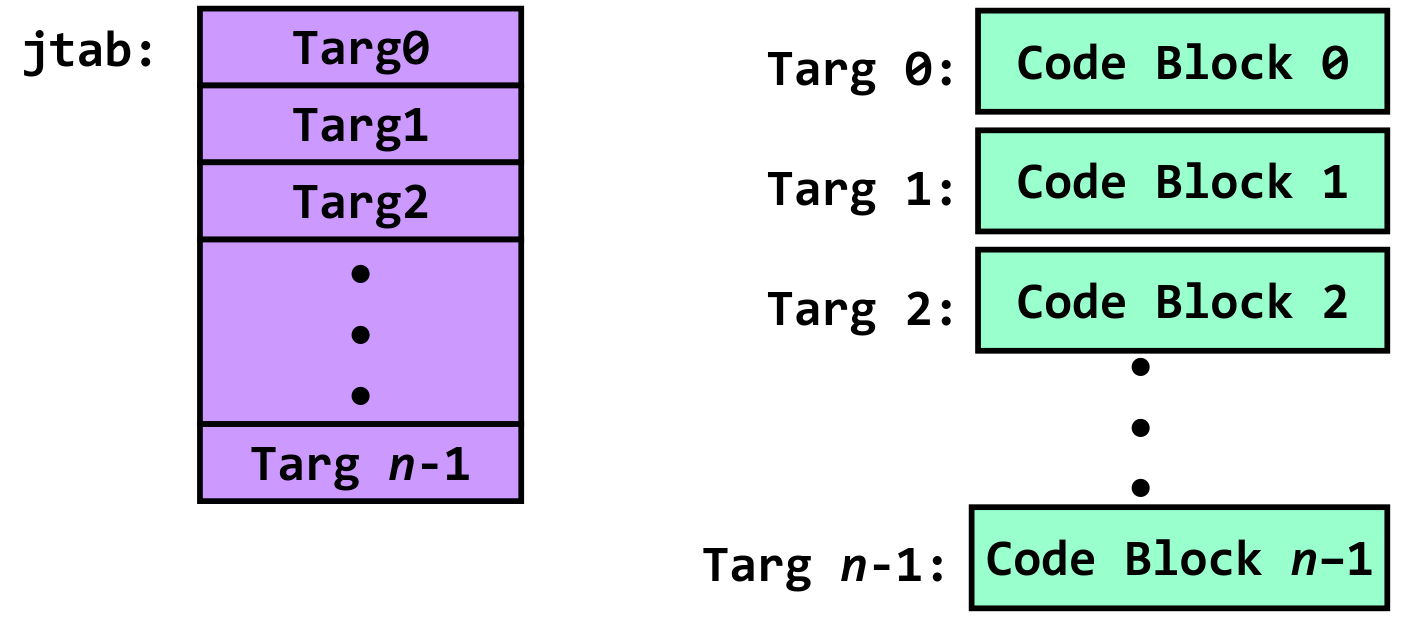
\includegraphics[width=10cm]{8.png}
    \caption{跳转表}
\end{figure}
翻译后(扩展 C)的形式为 \mintinline{c}{goto *JTab[op];},可通过跳转表快速根据 \mintinline{c}{x} 的值跳转到相应的代码块执行。


\subsubsection{分析跳转表}
以 \mintinline{c}{switch_eg} 函数为例:
\begin{minted}{c}
long switch_eg(long x, long y, long z) {
    long w = 1;
    switch(x) {
        ...
    }
    return w;
}
\end{minted}
其汇编代码如下:
\begin{minted}{asm}
setup: 
switch_eg:   
    movq    %rdx, %rcx 
    cmpq    $6, %rdi        # x:6 
    ja      .L8             # Use default if x > 6
    jmp     *.L4(,%rdi,8)   # goto *JTab[x] 
\end{minted}
其中,\mintinline{asm}{jmp *.L4(,%rdi,8)} 表示间接跳转到由 \mintinline{asm}{.L4} 开始的跳转表中索引为 \mintinline{c}{x}(\mintinline{asm}{%rdi} 存储 \mintinline{c}{x} 的值)的位置。当 \mintinline{c}{x} 大于 \mintinline{asm}{6} 时,会跳转到 \mintinline{asm}{.L8} 执行默认情况。注意,\mintinline{c}{w} 并没有在 \mintinline{c}{switch} 开始前初始化。

跳转表在汇编代码中的定义如下:
\begin{minted}{asm}
.section .rodata    # read-only data
    .align 8
.L4:
    .quad   .L8     # x = 0
    .quad   .L3     # x = 1
    .quad   .L5     # x = 2
    .quad   .L9     # x = 3
    .quad   .L8     # x = 4
    .quad   .L7     # x = 5
    .quad   .L7     # x = 6
\end{minted}
跳转表的基地址是 \mintinline{asm}{.L4},每个跳转目标需要 8 个字节(因为在 64 位系统中,地址是 8 个字节)。间接跳转时,缩放因子必须是 8 的整倍数,通过计算地址 \mintinline{asm}{.L4 + x * 8} 来获得跳转目标的位置(仅限于 \mintinline{asm}{0 <= x <= 6} 的情况)。

\subsubsection{代码块实现}
\begin{enumerate}
    \item \textbf{代码块(\mintinline{asm}{x == 1})}
          \begin{multicols}{2}
              \begin{minted}{asm}
.L3:
    movq    %rsi, %rax # y
    imulq   %rdx, %rax # y*z
    ret
    \end{minted}
              \columnbreak
              \begin{minted}{c}
        case 1:
            w = y*z;
            break;
    \end{minted}
          \end{multicols}
          当 \mintinline{c}{x} 等于 \mintinline{asm}{1} 时,执行此代码块,实现 \mintinline{c}{w = y*z} 的操作,其中 \mintinline{asm}{%rdi} 为参数 \mintinline{c}{x},\mintinline{asm}{%rsi} 为参数 \mintinline{c}{y},\mintinline{asm}{%rdx} 为参数 \mintinline{c}{z},\mintinline{asm}{%rax} 用于存储返回值。
    \item \textbf{处理落入另一个case的情况(\mintinline{asm}{x == 2,x == 3} )}
          \begin{multicols}{2}
              \begin{minted}{asm}
.L5:                    #Case2 
    movq    %rsi, %rax
    cqto
    idivq   %rcx        # y/z
    jmp     .L6         # goto merge 
.L9:                    # Case 3
    movl    $1, %eax    # w = 1
.L6:                    # merge:
    addq    %rcx, %rax  # w += z
    ret
    \end{minted}
              \columnbreak
              \begin{minted}{c}
        case 2:
            w = y/z;
            /* Fall Through */
        case 3:
            w += z;
            break;
    \end{minted}
          \end{multicols}

          对于 \mintinline{c}{case 2} 和 \mintinline{c}{case 3},\mintinline{c}{case 2} 执行完 \mintinline{c}{w = y/z} 后会继续执行 \mintinline{c}{case 3} 的代码,即跳转到 \mintinline{asm}{merge} 标签处执行 \mintinline{c}{w += z}。
    \item \textbf{代码块(\mintinline{c}{x == 5,x == 6} ,缺省)}
          \begin{multicols}{2}
              \begin{minted}{asm}
.L7:                    # Case 5,6
    movl    $1, %eax    # w = 1
    subq    %rdx, %rax  # w -= z
    ret
.L8:                    # Default:
    movl    $2, %eax    # 2
    ret
    \end{minted}
              \columnbreak
              \begin{minted}{c}
        case 5:
        case 6:
            w -= z;
            break;
        default:
            w = 2;
    \end{minted}
          \end{multicols}

          当 \mintinline{c}{x} 等于 \mintinline{asm}{5} 或 \mintinline{asm}{6} 时,执行 \mintinline{c}{w -= z};当 \mintinline{c}{x} 不满足任何 \mintinline{c}{case} 条件(即默认情况)时,执行 \mintinline{c}{w = 2}。
\end{enumerate}

\subsubsection{特殊情况处理}
\begin{enumerate}
    \item \textbf{没有从0处开始的情况}

          对于 \mintinline{c}{switch} 语句中 \mintinline{c}{case} 值不是从 \mintinline{asm}{0} 开始的情况,如:
          \begin{minted}{c}
void switch_eg_2(long x) {
    switch(x) {
        case 10000:
        ......
        case 10002:
        ......
        case 10005:
        ......
        default:
        ......
    }
}
    \end{minted}
          汇编代码会进行相应调整:
          \begin{minted}{asm}
switch_eg_2:
    leaq    -$10000(%rdi), %rsi     # %rsi = %rdi – 10000
    cmpq    $6, %rsi                # x:6
    ja      .L8                     # Use default
    jmp     *.L4(,%rsi,8)           # goto *JTab[x]
    \end{minted}
          通过 \mintinline{asm}{leaq -$10000(%rdi), %rsi} 将 \mintinline{c}{x} 的值进行调整,使其可以适配从 \mintinline{asm}{0} 开始索引的跳转表。
    \item \textbf{稀疏的switch语句}

          当 \mintinline{c}{switch} 语句的 \mintinline{c}{case} 值分布非常稀疏时,如:
          \begin{minted}{c}
switch(x) {
    case 0: 
            ...
    case 1000:
            ...
    case 92027:
            ...
}
    \end{minted}
          编译器可能会将其翻译为二分查找的语句(时间复杂度为 $O(\log n)$),而不是退化为逐个比较的 \mintinline{c}{if - else - if - else ...} 形式(时间复杂度为 $O(n)$),从而提高效率。
\end{enumerate}

\subsubsection{总结}
\mintinline{c}{switch} 语句通过条件跳转、间接跳转(利用跳转表实现)等机制实现其功能。编译器会根据 \mintinline{c}{switch} 语句的具体情况,如 \mintinline{c}{case} 值的连续性、数量等,自动生成合适的代码序列,以实现更复杂的控制逻辑。大规模的 \mintinline{c}{switch} 语句通常使用跳转表实现,而稀疏的 \mintinline{c}{switch} 语句则可以使用决策树(二分查找)来优化实现。

\section{程序的机器级表示:过程}

在计算机系统中,程序的机器级表示是理解程序如何在底层运行的关键。过程(函数调用)是程序设计中的重要概念,它涉及到控制流的转移、数据的传递以及栈的管理等多个方面。下面将详细介绍程序机器级表示中过程相关的知识。

\subsection{栈的结构}

\subsubsection{x86 - 64 的栈概述}

在 x86 - 64 架构的计算机系统中,栈是一种非常重要的数据结构,用于存储过程调用的上下文信息。栈的一个显著特点是它向低地址方向生长,这意味着当有新的数据入栈时,栈指针会向低地址移动。寄存器 \mintinline{asm}{%rsp} 用于存储栈的最低地址,也就是栈指针,它始终指向栈顶的位置。

栈的基本特性总结如下:
\begin{table}[H]
    \captionsetup{skip=4pt}
    \centering
    \setlength{\arrayrulewidth}{1pt}
    \begin{tabular}{c}
        \hline
        \makebox[0.8\textwidth][c]{栈的特性}             \\
        \noalign{\global\setlength{\arrayrulewidth}{0.5pt}}
        \hline
        栈底(Stack “Bottom”)位于高地址端,这是栈的起始位置。           \\
        栈顶(Stack “Top”)位于低地址端,随着数据的入栈和出栈,栈顶的位置会不断变化。 \\
        栈向下生长(Stack Grows Down),即向低地址方向扩展。当有新的数据需要入栈时,栈指针 \mintinline{asm}{%rsp} 会减小。 \\
        栈指针(Stack Pointer) \mintinline{asm}{%rsp} 始终指向栈顶,通过操作 \mintinline{asm}{%rsp} 可以实现数据的入栈和出栈操作。 \\
        \noalign{\global\setlength{\arrayrulewidth}{1pt}}
        \hline
    \end{tabular}
    \caption{x86 - 64 栈的基本特性}
\end{table}

\subsubsection{x86 - 64 的栈:入栈操作}

入栈操作 \mintinline{asm}{pushq src} 是将一个 64 位的数据从源操作数 \mintinline{asm}{src} 压入栈中。具体步骤如下:

\begin{enumerate}
    \item 从 \mintinline{asm}{src} 中取出操作数(Fetch operand at \mintinline{asm}{src}):首先,处理器会从源操作数 \mintinline{asm}{src} 所在的位置读取要入栈的数据。这个源操作数可以是寄存器或者内存地址。
    \item \mintinline{asm}{%rsp} 减 8(Decrement \mintinline{asm}{%rsp} by 8):由于在 x86 - 64 架构中,每个数据单元是 64 位(8 字节),所以在入栈时,栈指针 \mintinline{asm}{%rsp} 需要减去 8,以指向新的栈顶位置。
    \item 将操作数的值写入 \mintinline{asm}{%rsp} 指向的地址(Write operand at address given by \mintinline{asm}{%rsp}):最后,将从 \mintinline{asm}{src} 中取出的数据写入到新的栈顶位置,也就是 \mintinline{asm}{%rsp} 所指向的内存地址。
\end{enumerate}

下面是一个简单的入栈操作示例代码:
\begin{minted}{asm}
pushq %rax ; 将寄存器 %rax 中的值入栈
\end{minted}

在这个示例中,首先处理器会读取寄存器 \mintinline{asm}{%rax} 中的值,然后将栈指针 \mintinline{asm}{%rsp} 减 8,最后将 \mintinline{asm}{%rax} 中的值写入到新的栈顶位置。

\subsubsection{x86 - 64 的栈:出栈操作}

出栈操作 \mintinline{asm}{popq dest} 是将栈顶的 64 位数据弹出并写入到目标操作数 \mintinline{asm}{dest} 中。具体步骤如下:

\begin{enumerate}
    \item 从 \mintinline{asm}{%rsp} 指向的地址中取出值(Fetch value in \mintinline{asm}{%rsp}):处理器会从当前栈指针 \mintinline{asm}{%rsp} 所指向的内存地址读取栈顶的数据。
    \item 将值写入 \mintinline{asm}{dest}(Write value to operand \mintinline{asm}{dest}):将读取到的栈顶数据写入到目标操作数 \mintinline{asm}{dest} 中,目标操作数可以是寄存器或者内存地址。
    \item \mintinline{asm}{%rsp} 加 8(Increment \mintinline{asm}{%rsp} by 8):由于已经将栈顶的数据弹出,栈指针需要加 8,以指向新的栈顶位置。

\end{enumerate}

下面是一个简单的出栈操作示例代码:
\begin{minted}{asm}
popq %rbx ; 将栈顶的值弹出并写入寄存器 %rbx
\end{minted}

在这个示例中,处理器会先读取栈顶的值,然后将该值写入到寄存器 \mintinline{asm}{%rbx} 中,最后将栈指针 \mintinline{asm}{%rsp} 加 8。

\subsection{过程调用规范}

\subsubsection{控制流转移}

过程调用是程序中实现代码复用和模块化的重要手段。在 x86 - 64 架构中,过程调用通过 \mintinline{asm}{call label} 指令实现,而过程返回则使用 \mintinline{asm}{ret} 指令。

\mintinline{asm}{call label} 指令的执行过程如下:
\begin{enumerate}
    \item 将返回地址压入栈:返回地址是紧接在 \mintinline{asm}{call} 指令之后的指令所在的地址。当执行 \mintinline{asm}{call} 指令时,处理器会将这个返回地址压入栈中,以便在过程执行完毕后能够返回到正确的位置继续执行。
    \item 跳转至 \mintinline{asm}{label} 标签处的过程代码开始位置:处理器会跳转到 \mintinline{asm}{label} 所指定的地址处,开始执行被调用过程的代码。
\end{enumerate}

\mintinline{asm}{ret} 指令的执行过程如下:

\begin{enumerate}
    \item 从栈中弹出返回地址:处理器会从栈顶弹出之前压入的返回地址。
    \item 跳转至该地址:根据弹出的返回地址,处理器会跳转到相应的位置继续执行程序。
\end{enumerate}

下面是一个完整的过程调用示例代码:
\begin{minted}{asm}
; 示例代码:控制流转移
void multstore(long x, long y, long *dest) {
    long t = mult2(x, y);
    *dest = t;
}
0000000000400540 <multstore>:
    400540: push %rbx        # Save %rbx
    400541: mov %rdx,%rbx    # Save dest
    400544: callq 400550 <mult2> # mult2(x,y)
    400549: mov %rax,(%rbx)  # Save at dest
    40054c: pop %rbx        # Restore %rbx
    40054d: retq            # Return

long mult2(long a, long b) {
    long s = a * b;
    return s;
}
0000000000400550 <mult2>:
    400550: mov %rdi,%rax    # a 
    400553: imul %rsi,%rax   # a * b
    400557: retq            # Return
\end{minted}

在这个示例中,\mintinline{c}{multstore} 函数调用了 \mintinline{c}{mult2} 函数。当执行到 \mintinline{asm}{callq 400550 <mult2>} 指令时,会将下一条指令(\mintinline{asm}{400549})的地址压入栈中,然后跳转到 \mintinline{c}{mult2} 函数的起始地址(\mintinline{asm}{400550})开始执行。当 \mintinline{c}{mult2} 函数执行完毕,执行 \mintinline{asm}{retq} 指令时,会从栈中弹出返回地址(\mintinline{asm}{400549}),然后跳转到该地址继续执行 \mintinline{c}{multstore} 函数的后续代码。

\subsubsection{数据传递}

在 x86 - 64 架构中,数据传递遵循一定的规则。前 6 个参数通过寄存器传递,具体如下:

\begin{table}[H]
    \captionsetup{skip=4pt}
    \centering
    \setlength{\arrayrulewidth}{1pt}
    \begin{tabular}{c}
        \hline
        \makebox[0.8\textwidth][c]{用于传递参数的寄存器} \\
        \noalign{\global\setlength{\arrayrulewidth}{0.5pt}}
        \hline
        \mintinline{asm}{%rdi}:用于传递第一个参数。 \\
        \mintinline{asm}{%rsi}:用于传递第二个参数。 \\
        \mintinline{asm}{%rdx}:用于传递第三个参数。 \\
        \mintinline{asm}{%rcx}:用于传递第四个参数。 \\
        \mintinline{asm}{%r8}:用于传递第五个参数。 \\
        \mintinline{asm}{%r9}:用于传递第六个参数。 \\
        \noalign{\global\setlength{\arrayrulewidth}{1pt}}
        \hline
    \end{tabular}
    \caption{x86 - 64 中传递前 6 个参数的寄存器}
\end{table}

返回值通过 \mintinline{asm}{%rax} 寄存器传递。如果参数数量超过 6 个,剩余的参数则通过栈传递。并且,只有在需要时栈才会分配空间来存储这些额外的参数。

下面是一个参数传递的示例代码:
\begin{minted}{c}
long add_five_numbers(long a, long b, long c, long d, long e) {
    return a + b + c + d + e;
}

int main() {
    long result = add_five_numbers(1, 2, 3, 4, 5);
    return 0;
}
\end{minted}

对应的汇编代码中,参数 \mintinline{c}{1} 会被传递到 \mintinline{asm}{%rdi},参数 \mintinline{c}{2} 会被传递到 \mintinline{asm}{%rsi},参数 \mintinline{c}{3} 会被传递到 \mintinline{asm}{%rdx},参数 \mintinline{c}{4} 会被传递到 \mintinline{asm}{%rcx},参数 \mintinline{c}{5} 会被传递到 \mintinline{asm}{%r8}。函数执行完毕后,返回值会存储在 \mintinline{asm}{%rax} 中。

\subsubsection{存储管理}

在过程执行时,会为该过程分配栈帧空间。栈帧是栈中的一个区域,用于存储过程调用的相关信息,包括参数、局部变量、返回地址等。过程返回前,会释放栈帧空间,以便后续的过程调用使用。

栈帧的管理主要通过栈指针 \mintinline{asm}{%rsp} 和可选的帧指针 \mintinline{asm}{%rbp} 进行。栈指针 \mintinline{asm}{%rsp} 始终指向栈顶,而帧指针 \mintinline{asm}{%rbp} 可以指向栈帧的底部,方便访问栈帧中的数据。

栈帧的内容通常包括以下几个部分:
\begin{table}[H]
    \captionsetup{skip=4pt}
    \centering
    \setlength{\arrayrulewidth}{1pt}
    \begin{tabular}{cc}
        \hline
        \makebox[0.4\textwidth][c]{栈帧内容}    & \makebox[0.4\textwidth][c]{说明}                                                        \\
        \noalign{\global\setlength{\arrayrulewidth}{0.5pt}}
        \hline
        参数(Arguments)                       & 即将要调用的函数的参数或本次调用的参数。如果参数数量超过 6 个,超出部分会存储在栈帧中。                                         \\
        本地变量(Local variables)               & 在寄存器中保存不下的变量。例如,一些数组或者复杂的数据结构通常会存储在栈帧中。                                               \\
        保存的寄存器上下文信息(Saved register context) & 保存过程中使用的寄存器的值,以便恢复。当一个过程需要使用某些寄存器,但又不希望破坏这些寄存器原来的值时,会将这些寄存器的值保存到栈帧中,在过程返回前再恢复。        \\
        指向调用者的栈帧底部的指针(Old frame pointer,可选) & 用于回溯调用栈,可用于访问调用者栈帧中的数据。通过帧指针 \mintinline{asm}{                                        %rbp} 可以方便地找到调用者的栈帧,从而实现对调用者栈帧中数据的访问。 \\
        返回地址(Return address)                & 调用 \mintinline{asm}{call} 指令时入栈,用于过程返回时跳转。当过程执行完毕,需要返回到调用者继续执行时,会从栈帧中取出返回地址,然后跳转到该地址。 \\
        \noalign{\global\setlength{\arrayrulewidth}{1pt}}
        \hline
    \end{tabular}
    \caption{x86 - 64/Linux 栈帧内容}
\end{table}

\subsubsection{寄存器使用惯例}

在 x86 - 64 架构中,寄存器分为“调用者保护”和“被调用者保护”两类,这是为了保证在过程调用过程中寄存器的值不会被意外修改。

“调用者保护”的寄存器,调用者在调用前把临时数据保存到自己的栈帧中。这意味着,如果一个过程(调用者)需要使用这些寄存器,并且希望在调用其他过程后这些寄存器的值仍然保持不变,那么它需要在调用之前将这些寄存器的值保存到自己的栈帧中,在调用返回后再恢复这些值。

“被调用者保护”的寄存器,被调用者在使用前将临时数据保存至自己的栈帧中,并在返回前恢复这些数据。也就是说,当一个过程(被调用者)需要使用这些寄存器时,它需要先将这些寄存器的值保存到自己的栈帧中,在使用完后再恢复这些值,以确保调用者看到的这些寄存器的值没有被改变。

具体的寄存器分类如下:
\begin{table}[H]
    \captionsetup{skip=4pt}
    \centering
    \setlength{\arrayrulewidth}{1pt}
    \begin{tabular}{cc}
        \hline
        \makebox[0.4\textwidth][c]{寄存器类别} & \makebox[0.4\textwidth][c]{寄存器列表} \\
        \noalign{\global\setlength{\arrayrulewidth}{0.5pt}}
        \hline
        调用者保护(Caller - saved)             & \mintinline{asm}{                 %rax}, \mintinline{asm}{%rdi}, \mintinline{asm}{%rsi}, \mintinline{asm}{%rdx}, \mintinline{asm}{%rcx}, \mintinline{asm}{%r8}, \mintinline{asm}{%r9}, \mintinline{asm}{%r10}, \mintinline{asm}{%r11} \\
        被调用者保护(Callee - saved)            & \mintinline{asm}{                 %rbx}, \mintinline{asm}{%r12}, \mintinline{asm}{%r13}, \mintinline{asm}{%r14}, \mintinline{asm}{%rbp}, \mintinline{asm}{%rsp} \\
        \noalign{\global\setlength{\arrayrulewidth}{1pt}}
        \hline
    \end{tabular}
    \caption{x86 - 64 Linux 中寄存器的保护类别}
\end{table}

下面是一个寄存器使用惯例的示例代码:
\begin{minted}{c}
void function1() {
    long temp = 10;
    function2();
    // 此时 temp 的值仍然是 10,因为 %rax 是调用者保护寄存器
}

void function2() {
    long result = 20;
    // 可以安全地使用 %rax 寄存器,因为调用者已经保存了 %rax 的值
    // ...
}
\end{minted}

在这个示例中,\mintinline{c}{function1} 是调用者,\mintinline{c}{function2} 是被调用者。如果 \mintinline{c}{function1} 需要使用 \mintinline{asm}{%rax} 寄存器,并且希望在调用 \mintinline{c}{function2} 后 \mintinline{asm}{%rax} 的值不变,那么它需要在调用之前保存 \mintinline{asm}{%rax} 的值。而 \mintinline{c}{function2} 可以安全地使用 \mintinline{asm}{%rax} 寄存器,因为调用者已经处理了 \mintinline{asm}{%rax} 的保存和恢复。

\subsection{递归}

递归是一种函数调用自身的编程技术,它在解决一些复杂问题时非常有用。下面以计算无符号长整型数中 1 的个数的递归函数 \mintinline{c}{pcount_r} 为例进行说明。

\subsubsection{递归函数的代码实现}

\begin{minted}{c}
/* Recursive popcount */
long pcount_r(unsigned long x) {
    if (x == 0)
        return 0;
    else
        return (x & 1) + pcount_r(x >> 1);
}
\end{minted}

这个函数的功能是计算无符号长整型数 \mintinline{c}{x} 中二进制表示下 1 的个数。如果 \mintinline{c}{x} 为 0,则返回 0;否则,返回 \mintinline{c}{x} 的最低位(\mintinline{c}{x & 1})加上 \mintinline{c}{x} 右移一位后剩余部分中 1 的个数(通过递归调用 \mintinline{c}{pcount_r(x >> 1)} 计算)。

\subsubsection{递归函数的汇编代码分析}

对应的汇编代码如下:
\begin{minted}{asm}
pcount_r:
    movl $0, %eax
    testq %rdi, %rdi
    je .L6
    pushq %rbx
    movq %rdi, %rbx
    andl $1, %ebx
    shrq %rdi # (by 1)
    call pcount_r
    addq %rbx, %rax
    popq %rbx
.L6:
    rep; ret
\end{minted}

下面对这段汇编代码进行详细分析:
\begin{enumerate}
    \item \mintinline{asm}{movl $0, %eax}:将寄存器 \mintinline{asm}{%eax} 初始化为 0,用于存储最终的结果。
    \item \mintinline{asm}{testq %rdi, %rdi}:对寄存器 \mintinline{asm}{%rdi} 进行按位与操作,用于判断 \mintinline{asm}{%rdi} 是否为 0。如果为 0,则设置相应的标志位。
    \item \mintinline{asm}{je .L6}:如果 \mintinline{asm}{%rdi} 为 0(即 \mintinline{c}{x} 为 0),则跳转到标签 \mintinline{asm}{.L6} 处,直接返回 0。
    \item \mintinline{asm}{pushq %rbx}:将寄存器 \mintinline{asm}{%rbx} 的值压入栈中,因为 \mintinline{asm}{%rbx} 是被调用者保护寄存器,需要在使用前保存其值。
    \item \mintinline{asm}{movq %rdi, %rbx}:将参数 \mintinline{c}{x}(存储在 \mintinline{asm}{%rdi} 中)复制到寄存器 \mintinline{asm}{%rbx} 中。
    \item \mintinline{asm}{andl $1, %ebx}:对 \mintinline{asm}{%ebx} 的最低位进行按位与操作,得到 \mintinline{c}{x} 的最低位。
    \item \mintinline{asm}{shrq %rdi}:将 \mintinline{asm}{%rdi} 中的值右移一位,相当于 \mintinline{c}{x >> 1}。
    \item \mintinline{asm}{call pcount_r}:递归调用 \mintinline{c}{pcount_r} 函数,计算 \mintinline{c}{x >> 1} 中 1 的个数。
    \item \mintinline{asm}{addq %rbx, %rax}:将 \mintinline{c}{x} 的最低位(存储在 \mintinline{asm}{%rbx} 中)加到结果寄存器 \mintinline{asm}{%rax} 中。
    \item \mintinline{asm}{popq %rbx}:从栈中弹出之前保存的 \mintinline{asm}{%rbx} 的值,恢复 \mintinline{asm}{%rbx} 的原始值。
    \item \mintinline{asm}{rep; ret}:返回调用者,将结果存储在 \mintinline{asm}{%rax} 中。
\end{enumerate}

递归函数的处理和普通函数调用类似,栈帧为每次函数调用提供私有的存储空间,用于保存寄存器和局部变量、返回地址等。寄存器使用惯例保证了一次函数调用不会破坏其他函数的数据,栈的后进先出特性也适用于递归和相互递归的情况。


\end{document}